\documentclass[10pt,twoside]{book}

\usepackage{graphicx}
\usepackage{booktabs}
\usepackage{color}
\usepackage{colortbl}

\oddsidemargin=-5mm
\evensidemargin=-5mm
\topmargin=-5mm
\textwidth=170mm
\textheight=240mm

\pagestyle{myheadings}

\markboth{\dotfill MeqTree Kernel Design Overview}{\small\tt
LOFAR/doc/MEQ/MeqDesignOverview.tex\em~~$\circ$~$ $Revision$ $~$\circ$~$ $Date$ $\dotfill}

\title{{\sf MeqTree Kernel Design Overview (PSS4)}}

\author{{\sf O.M. Smirnov}}

\date{\vspace{2cm}\small CVS path: \tt LOFAR/doc/MEQ/MeqDesignOverview.tex\\\rm
$ $Revision$ $\\$ $Date$ $}

\begin{document}

\sloppy


\maketitle
\tableofcontents

% \qq{text} used to quote code (in fixed font)
\newcommand{\qq}[1]{{\tt #1}}

% \url{text} inserts a URL
\newcommand{\url}[1]{{\tt #1}}

% commands for some common Meq-terms
\newcommand{\Request}{{\tt Request}}
\newcommand{\RequestId}{{\tt RequestId}}
\newcommand{\Result}{{\tt Result}}
\newcommand{\VellSet}{{\tt VellSet}}
\newcommand{\Cells}{{\tt Cells}}
\newcommand{\Vells}{{\tt Vells}}
\newcommand{\Domain}{{\tt Domain}}
\newcommand{\Node}{{\tt Node}}
\newcommand{\Parm}{{\tt Parm}}
\newcommand{\Polc}{{\tt Polc}}
\newcommand{\RES}[1]{{\tt RES\_#1}}

% math symbols: real numbers, complex numbers, P for parameter space
\newcommand{\RR}{\mathcal{R}}
\newcommand{\CC}{\mathcal{C}}
\newcommand{\PP}{\mathcal{P}}

% define some standard colors
\definecolor{tableheading}{rgb}{0.8,0.85,1}
\definecolor{tabletext}{gray}{0}
\definecolor{tablesubheading}{gray}{.9}
%
\definecolor{highlight}{rgb}{1,1,0}

% this command creates a paragraph with a highlit background, separated
% by extra space from surrounding paragraphs.
\newcommand{\highlightbox}[1]{\smallskip\noindent\colorbox{highlight}{\parbox{\textwidth}
{\noindent #1}}\smallskip}%
% \addvspace{\smallskipamount}}

% \tablesubheading{n}{text} inserts a sub-heading into a table.
% n argument is the number of columns that the sub-heading will span

  \newlength{\taboverhang}
  \setlength{\taboverhang}{\tabcolsep}
  \addtolength{\taboverhang}{-1pt}

\newcommand{\tablesubheading}[2]%
{\multicolumn{#1}{|>{\columncolor{tablesubheading}}l|}{\strut\em~~~~~#2}}

% \standardtableheading produces a standard heading for tables
% field name | type | description
\newcommand{\standardtableheading}[1]%
{\rowcolor{tableheading}#1\\}

% \recordtableheading produces a standard heading for record tables:
% field name | type | description
\newcommand{\recordtableheading}
{\standardtableheading{\sl field name & \sl type & \sl description}}

% \statetableheading produces a standard heading for state tables:
% field name | type | default | description
\newcommand{\statetableheading}
{\standardtableheading{\sl field name & \sl type & \sl default & \sl description}}


\arrayrulecolor{tableheading}

% \recordtableentry{name}{type}{desc} produces one line
% of a record layout table
\newcommand{\recordtableentry}[3]
{\color{tabletext}\qq{#1} & \qq{#2} & #3\\}

% \statetableentry{name}{type}{default}{desc} produces one line
% of a state record layout table
\newcommand{\statetableentry}[4]
{\color{tabletext}\qq{#1} & \qq{#2} & \qq{#3} & #4\\}

\chapter{The Fundamentals}

  The purpose of this document is to provide an in-depth description of the
  MeqTree kernel and related interfaces. The following subjects will be
  covered:

  \begin{itemize}

  \item Basic terms and concepts.

  \item System components.

  \item Data structures employed in the MeqTree kernel.

  \item Standard node state \& functionality.

  \item Interaction between nodes, and how it is affected by state.

  \item Interaction with Glish (and in the future, other scripting languages).

  \item Examples of some standard and application-specific nodes.

  \end{itemize}

  The intended audience for this document is:

  \begin{description}

  \item[The Tree Designer,] since a thorough understanding of how nodes interact
  is critical in construction of complex and efficient trees.

  \item[The Node Developer] needing to implement specialized node classes.

  \end{description}


\section{Trees}

  The MeqTree kernel provides a C++ implementation of the MeqTree concept. A {\bf
  MeqTree} (or simply ``tree'') is a collection of interconnected {\bf MeqNodes}
  (or simply ``nodes''). Nodes have a directed parent--child relationship; a
  parent may have any number of children, and a child can have multiple parents.
  Cycles are forbidden. Technically, this makes the MeqTree a {\em directed
  acyclic graph}, but the term ``tree'' is retained for historical and
  aesthetical reasons.

  We will often use directional terms when discussing trees, {\bf up} is from
  parent to child, and {\bf down} is from child to parent.

  In broad terms, the life of a node generally consists of receiving {\bf
  requests} from its parent(s), passing them up to its children, receiving {\bf
  results} in response, performing some calculation on the child results, and
  returning the result down to its parent(s). Thus, requests generally originate
  somewhere down the tree and propagate up, while results germinate at the top
  and percolate down. 

\section{The math}
  \label{sec:math}

  Trees are mostly concerned with evaluating functions (e.g., predicted
  visibilities), optionally comparing these functions to other functions (e.g.,
  measured visibilities), and solving for adjustable parameters to obtain the
  best fit. Before we discuss this in detail, it helps to define some basic 
  mathematical terms.

  The result of a node usually represents some function defined over
  $\mathcal{R}^2$ space -- $f:\RR^2\rightarrow\RR^N$ or
  $f:\RR^2\rightarrow\CC^N$. The $\mathcal{R}^2$ domain is interpreted as
  frequency--time space in our application context, but in fact there's very
  few places in the kernel where this has any specific meaning. The codomain,
  $\RR^N$ or $\CC^N$, could represent any number of things, e.g., a single
  correlation $XX\in\CC$, the Stokes parameters $(IQUV)\in\RR^4$, four complex
  correlations in $\CC^4$, etc.

  The actual function {\bf domain} $[X_1,X_2]\times[Y_1,Y_2]$  is a rectangular
  subset of $\RR^2$. This domain is fully or partially covered  by a set of
  $N\times M$ {\bf cells}. Each cell ${\mathbf c}_{ij}$ is a $\Delta
  x_i\times\Delta y_j$ rectangle, centered on point $(x_i,y_j)$. The function
  itself is represented by an object called the {\bf vells}, which is
  essentially a set of $N\times M$ {\em samplings}\/ $\bar{f}=\{f_{ij}\}$: 
  $$f_{ij}=f(x_i,y_j),$$ or $N\times M$ {\em integrations}\/
  $\bar{f}=\{\tilde{f}_{ij}\}$: $$
  \tilde{f}_{ij}=\mathop{\int\!\!\!\int}_{{\mathbf c}_{ij}}f(x,y)\,dx\,dy.$$

  A vells $\bar{f}=\{f_{ij}\}$ can also represent a set of {\em measured data}, such as
  observed complex visibilities. 
  
  A function may also depend on $K$ real parameters. If we designate the {\em
  parameter space} $\PP:=\RR^K$, then our function essentially becomes
  $f:\RR^2\times\PP\rightarrow\RR^N$ or $f:\RR^2\times\PP\rightarrow\CC^N$.
  This can also be represented as $f(x,y;p_1...p_K)$, or $f(x,y;\vec{p})$. The
  {\em model fitting problem} is essentially a minimization problem: finding
  the value $\vec{p}_0$  that minimizes the function $\chi^2(x,y;\vec{p})$ over
  a fixed set of cells in $(x,y)$ space. The $\chi^2$ function  ties together
  {\em predict function} $f(x,y;\vec{p})$, measured data $\{\hat{f}_{ij}\}$, and
  an optional set of weights $\{w_{ij}\}$:

  $$ \chi^2(\vec{p}) = \sum_{ij} (f(x_i,y_j;\vec{p}) - \hat{f}_{ij})^2w_{ij},$$
  
  Solving the minimization problem hinges on estimating the gradients of $f$ in
  $\PP$ space.\footnote{The exact mathematical expressions are slightly
  different when dealing with integrations (as we do in the case of
  visibilities), but most operations remain essentially the same.} Given a tree
  that computes $f_{ij}=f(x_i,y_j;\vec{p})$, we can numerically estimate each
  partial derivative ${\partial f}/{\partial p_k}(x,y;\vec{p})$ by taking a
  small {\bf perturbation} $\delta_k$, and using the same tree to compute a
  {\bf perturbed value} for parameter $k$: $f^{(k)}_{ij} =
  f(x_i,y_j;p_1,...,p_{k-1},p_k+\delta_k,p_{k+1},...,p_{K})$. In fact, the
  kernel is designed to automatically compute perturbed values when needed.
  More precise estimates may be obtained by using two sets of perturbed values
  (``double-differencing''), with different perturbations $\delta^{(1)}_k$ and
  $\delta^{(2)}_k$ (generally, $\delta^{(2)}_k = - \delta^{(1)}_k$). The
  different sets of perturbed values are designated as $f^{(sk)}_{ij} (s=1,2)$.
  These are passed around as a {\bf vellset}, which is composed of the {\em
  value vells} $\{f_{ij}\}$, $K\times S (S=1,2)$ {\em perturbed value vells}
  $\{f^{(sk)}_{ij}\}$, and $S$ vectors of  the perturbation themselves
  ${\delta^{(s)}_k}$.


\section{Nodes}

  Nodes are implemented as C++ objects, subclassed from the abstract
  \qq{Meq::Node} class\footnote{All the MeqTree kernel classes reside in the
  \qq{Meq} namespace; we will omit \qq{Meq::} from names from now on.}. All
  interaction with nodes is done via the \Node\ class interface. Consequently, a
  node has no direct knowledge of the {\em type} of its children. Nodes may be
  connected together in a practically arbitrary manner. Given a rich toolbox of
  elementary node classes, trees representing arbitrary mathematical expressions
  may thus be constructed. 

  All nodes have a {\bf state record} that determines their behaviour. The state
  record is fully accessible from the outside. The initial state record is also
  called the {\bf defrec} (from definition record), and is usually supplied from
  the scripting layer when the node is created.

  Nodes also have a {\bf result cache} that may retain the most recently computed
  result. The cache is intended to save processing time for repeated (or similar
  enough) requests.

\section{Design Philosophy}

  These principles are key to understanding the design philosophy behind the
  kernel:

  \begin{description}

  \item[Locality:] all functionality is defined in terms of local parent--child
  request--result interactions. There is no centralized ``control'' as such.

  \item[KISS and rely on emergent behaviour:] complex behaviour of the tree as
  a whole emerges from primitive request--result interactions at the local
  level. Most node classes are designed to be simple (K.I.S.S.!), with a single
  well-defined purpose. If some sort of specific functionality is required, it
  is almost always preferrable to implement it by building the right tree,
  rather than developing specialized nodes.

  \item[Policy-free:] kernel node classes are largely policy-free. By policy we
  mean any sort of application-specific behaviour or concepts. Policy may only
  emerge at the tree level (by connecting the nodes in a specific way), and/or
  at the scripting level.

  \item[Prohibition is for policy-makers:] this is a corollary to the
  previous principle. Apart from minimal and obvious sanity checks, the kernel
  imposes very few restrictions on its interface calls. This, of course, is a
  double-edged sword -- it provides great power, but also great opportunities
  to do something wrong. It is left to the higher-level (i.e.
  application-level) scripting code to shackle the user and protect him from
  mistakes.

  \item[There is more than one way to do it:] (with a nod to Larry Wall and
  Perl) in a lot of cases, the kernel provides several ways of accomplishing
  the same  result. There is not necessarily a single ``right'' way, it all
  depends on the particular application context. This redundancy is by design,
  as it increases the overall adapatability of the system.

  \end{description}

\section{Software components}

  An interface to the kernel is provided via a \qq{MeqServer} object. The
  \qq{MeqServer} maintains a \qq{Forest} (a collection of nodes and trees), and
  provides operations such as:

  \begin{itemize}

  \item Create, connect and delete node objects.

  \item Inspect and modify node state records.

  \item Issue requests and return results.

  \item Connect trees to data sources (e.g. Measurement Sets).

  \end{itemize}

  \qq{MeqServer} plugs into the OCTOPUSSY publish/subscribe framework, and
  through it can can transparently support any number of local or remote
  clients, such as Glish sessions. The \qq{MeqServer} object is instantiated
  inside a \qq{meqserver} process.

  All application-dependent logic (``policy'') is meant to reside in the scripting
  layer (Glish, and in the future Python).

\chapter{Data Structures} 

\section{Basic concepts}

  The main priciple driving data structure design in MeqTrees is {\bf
  congruity}: all C++ objects used to {\em pass information} within a tree must
  be mappable without any loss of information to and from data structures on
  the scripting side. Fully {\em private} structures (e.g., private nested
  classes) can exist on the C++ side only.

  Congruity facilitates {\bf transparency}: most of the inner workings of a
  tree are readily accessible from the scripting side. This allows for very
  elaborate monitoring schemes, and is a great debugging aid when something
  goes wrong.

\subsection{Data types}
  
  The choice of atomic data types is limited by the requirement of congruity.
  Currently, the only supported scripting language is Glish, but Python 
  support is expected in the near future. In any case, the kernel  restricts
  itself to common primitives that are supported by all mature scripting
  languages. Thus, kernel data structures are defined in terms of a restricted
  set of ``legal data objects'', specifically:

  \begin{itemize}
  
  \item scalars -- bool, integer, float, double, float or double complex;
  
  \item strings;
  
  \item multidimensional arrays of scalars;
  
  \item lists of legal objects (in Glish this is represented either  via a
  vector of scalars or strings, or via a record with fields indexed by number);

  \item records of legal objects (a.k.a. dictionaries/maps/hashes with a string
  key and a legal object value).

  \end{itemize}

  On the C++ side, data objects are based on the DMI \qq{DataRecord},
  \qq{DataField} and \qq{DataArray} classes. Most data classes are in fact
  derived from \qq{DataRecord}, and are at core a record with some (sometimes
  loosely) predefined structure.

\subsection{HIIDs}

  The \qq{HIID} (hierarchical indentifier) class of the DMI package is used for
  all data-related indentifiers in the kernel, such as record fields, node
  groups, request IDs, etc.
  
  A HIID is essentially a vector of integers called {\em atomic IDs}. Atomic
  IDs have a string representation: for IDs $>=$0 this is simply the integer
  itself in string form, while for IDs $<$0, a global {\em dictionary} (i.e.
  map from strings to numbers) is maintained in the development tree. Another
  way to look at this is that negative IDs represent {\em atomic concepts}, or
  words. Thus, any HIID can be viewed as a mix of words (from a fixed though
  rather large vocabulary!) and numbers.

  The string form of a HIID consists of atomic IDs, separated by periods. For
  example, \qq{"Request.ID.1"} is the string form of $(-1210,-1087,1)$. Note
  that the string form is {\bf not} case-sensitive, so \qq{"request.id.1"}
  corresponds to the same HIID. An alternative string representation, employing
  underscore (\qq{"\_"}) as the separator, is used for Glish record fields,
  e.g., \qq{rec.request\_id\_1}. 

  The reason we use HIIDs instead of plain strings is efficiency on the
  C++ side -- many data storage classes engage in parsing or building up HIIDs,
  and vectors of integers are much easier to manipulate than strings. Note that
  the symbol-to-ID mapping is also available as C++ header files containing
  \qq{const} declarations for atomic IDs. These may be used as, e.g.:

  \begin{verbatim}
  const HIID MyFieldName = AidRequest | AidId | 1;
  \end{verbatim}
  
  which is a convenient and visually obvious way to define a constant HIID
  corresponding to \qq{"Request.ID.1"}. The compiler turns this declaration
  into a \qq{const HIID} object -- essentially, a constant vector of integers.

  HIIDs are covered in more detail in the documentation for DMI. Here we'll
  only dwell on their Glish form. There's two forms in which HIIDs appear in
  Glish:
  
  \begin{itemize}
  
  \item As record field names, e.g., \qq{rec.request\_id}. The implication of
  this is that in order to be recognized by the kernel, all record field names
  must be built up from a fixed vocabulary (which may be extended by the
  C++ developer as new classes are added).

  \item As values. In Glish, a HIID value is just a string containing the
  HIID's symbolic form, tagged by the \qq{::is\_dmi\_hiid} attribute. The
  \qq{hiid()} function (in \qq{dmitypes.g}) is a convenient way to create HIID
  values. For example:

  \begin{verbatim}
  my_id := hiid('Request.ID.1');
  my_id := hiid('request','id',1);
  \end{verbatim}
  
  will both create the same HIID. 
  
  Note the crucial difference between strings and HIID values. Compare the two
  Glish records:

  \begin{verbatim}
  rec1 := [ a = 'a.b.c.1' ];
  rec2 := [ a = hiid('a.b.c',1) ];
  \end{verbatim}
  
  While they may appear to be practically identical on the Glish side of things
  -- both records contain the string field \qq{a}, except \qq{rec2.a} has an
  extra attribute tag -- when passed to the C++ kernel, \qq{rec1.a} is
  converted to an \qq{std::string} object, while \qq{rec2.a} is converted to a
  \qq{HIID} object.
  
  \end{itemize}

  In this document, we will use both forms interchangably depending on context,
  with the understanding that, e.g., \qq{request\_id\_1} and \qq{"Request.ID.1"}
  both refer to the thing as far as the kernel is concerend.

\subsection{Naming conventions}

  \begin{itemize}

  \item In C++, standard data structures \& nodes reside in \qq{namespace Meq}.
    In Glish, corresponding object constructor functions are placed into the
    {\tt meq} ``namespace'' (actually just a record), and names are
    all-lowercase. The DMI dynamic type system uses a {\tt Meq} prefix for the
    namespace. Thus, the \qq{Meq::\Request} class in C++ is registered as a
    ``\qq{MeqRequest}'' in the DMI type system, and  has a \qq{meq.request()}
    counterpart in Glish.

  \item Even though the languages we use are case-sensitive, HIIDs aren't. A
    good reason to avoid relying on character case to distinguish identifiers is
    that different languages and contexts have different capitalization
    conventions -- compare, e.g., \qq{Meq::Request} in C++, as opposed to
    \qq{meq.request} in Glish. Thus we should always avoid assigning
    case-sensitive names to different entities.

  \end{itemize}

\subsection{Glish \qq{meq} objects: meqtypes.g}

  With a couple of exceptions, Meq objects are represented by Glish records of
  a [mostly] predefined layout. The Glish/C++ conversion layer uses a few
  ``magic'' attributes to distinguish these objects from ordinary records, so
  it is able to map them to specialized Meq C++ classes rather than generic
  \qq{DataRecord}s. 

  Specifically, the \qq{::dmi\_actual\_type} attribute is set to a string which
  gives the DMI object type. Thus, it is possible to construct a record in
  Glish, tag it with \qq{::dmi\_actual\_type}, pass it thorugh the Glish/C++
  layer, and have it auto-magically converted to an C++ object of the
  appropriate class. The only requirement is that the record contain the
  correct set of fields, which are mapped to class attributes (data members) in
  C++. In practice, it's a lot more convenient to use the ``constructor''
  functions defined in \qq{meq/meqtypes.g}, which create properly formed and
  tagged records\footnote{Note that some Meq classes may have Glish
  counterparts but no Glish constructors. At time of writing, these include
  \Vells, \VellSet{}s, and \Result{}s. The reason for this is simply lack of
  necessity, since objects of these classes always originate on the C++ side
  rather than Glish. In the future, constructors for these classes may be added
  to Glish as required.}:

  \begin{description}
  
  \item[\qq{meq.domain()}] creates a Domain object (record).

  \item[\qq{meq.cells()}] creates a Cells object (record).

  \item[\qq{meq.requestid()}] creates a request ID from individual components
  (e.g., domain ID, config ID, iteration ID). A request ID is really just a
  \qq{HIID}.

  \item[\qq{meq.request()}] creates a Request object (record).
  
  \item[\qq{meq.polc()}] creates a Polc object (record).
  
  \end{description}
  
  In general, all data objects on the C++ side have counterparts on the Glish
  side. Within this document, we will usually describe data objects in terms of
  their Glish equivalents -- records and record fields -- with the implied
  understanding that there is a 1:1 mapping from that to C++ classes and data
  members.

\subsection{Glish lists}

  Glish does not have a native ``list'' (a.k.a. ``sequence'') type.
  Instead, lists are emulated in one of two ways:

  \begin{itemize}

  \item If all list elements are all of the same {\em scalar} type,
  then the list is emulated by a vector.
  
  \item If the list elements are of a non-scalar type, or the type is not
  homogenous, then the list is emulated by a record.\footnote{When mapping lists created
  in the kernel to Glish records, the conversion layer assigns field names of
  the form \qq{"\#1"}, \qq{"\#2"}, etc.}
  \end{itemize}

  Since Glish records support numeric subscripts, both types of lists can be
  accessed via the same syntax -- \qq{len(list)} returns the number of
  elements, \qq{list[$n$]} accesses element $n$. Note though that if a list
  contains only one element, it should still be accessed as \qq{list[1]} rather
  than \qq{list} (the latter syntax will actually do the right thing given a
  vector, but not a record, hence it should be avoided for consistency's sake.)
  
  We will use the term {\em list} from now on to refer to both types of Glish
  structures, as it should usually be clear from context which type is actually
  employed.


\subsection{1-based and 0-based indexing}
  \label{sec:01base}
  \label{sec:indexconv}

  Glish array indices are 1-based, while C++ indices are 0-based. This,
  unfortunately, has always led to all sorts of confusion, since indices pop up
  on both sides of the Glish/C++ barrier, and sometimes even need to be passed
  back and forth. As our experience with AIPS++ has shown, keeping track of
  index conversion on an individual basis is completely impractical.

  \highlightbox{The Glish/C++ conversion layer attempts to address this issue by
  providing {\em automatic conversion} of indices. If a record field's name
  ends in \qq{\_index} (on the C++ side this corresponds to a field HIID ending
  in the atomic ID \qq{"Index"}), and the field contains a single integer or a
  list of integers, then the field is assumed to contain indices, and
  conversion between 0- and 1-base is automatically performed.}

  Thus, the Glish record \qq{[foo=1,foo\_index=1,bar\_index=[2,3]]} will be
  converted to \qq{[Foo=1,Foo.Index=0,Bar.Index=[1,2]]} on the C++ side (and
  vice versa), while \qq{[foo\_index=1.0]} or \qq{[foo\_index=[a=1,b=2]]} will
  not undergo any conversion (since the \qq{\_index} field contains a
  \qq{double} value in one case, and a subrecord in the other case).

  Automatic conversion, of course, introduces its own potential for confusion
  if forgotten about. This is why you simply shouldn't forget about it. 

\section{MeqRequest and related data objects}
  \label{sec:request}

  A \Request\ is a {\em job description} containing a number of commands that a
  node executes in order to produce a \Result. A \Request\ is implemented as a
  record with a semi-fixed structure; commands correspond to specific field 
  names, while the value of each field usually carries the command arguments.
  
  Operationally, the critically important command is \qq{cells}: this tells the
  node to evaluate itself over a given grid in the frequency--time domain. In
  fact, most other commands are mere housekeeping, while \qq{cells} represents
  the brunt of the workload. For this reason, the \qq{cells} command gets
  special treatment: it is placed at the top level of the request record (along
  with a few related flags), and all nodes are obliged to process it. All other
  commands are kept inside a {\bf rider} sub-record, and are subject to a {\em
  node selection} mechanism that allows commands to be directed to all nodes,
  individual nodes, or groups of nodes (this is described in further detail in
  section~\ref{sec:CSR}).

  Each \Request\ is assigned a unique request ID ({\bf rqid}, pronounced
  ``arr-cue-d''). This is a \qq{HIID} describing various properties of the
  request. Request generators are expected to follow a certain {\em contract},
  and assign rqids in a consistent way. This is covered in detail in
  section~\ref{sec:rqid-contract}.

  On the C++ side, a \Request\ is derived from \qq{DataRecord}. It can contain
  the following fields (of which only \qq{request\_id} is obligatory).
  \vspace{1em}

  \noindent
  \begin{center}\begin{tabular}{|llp{.7\textwidth}|}
  \recordtableheading\addlinespace
  \recordtableentry{request\_id}{HIID}{the request ID}
  \recordtableentry{cells}{Cells}{{\em [optional]}~~a \Cells\ object (see
    below)}
  \recordtableentry{calc\_deriv}{int}{{\em [optional]}~~compute perturbed values (0, 1 or 2).
    Default is 0.}
  \recordtableentry{next\_request}{\rm ---}{{\em [optional]}~~a hint of what the
    next request is going to be. This influences caching decisions and
    speculative execution (section~\ref{sec:nextreq}). {\em Placeholder only,
    not currently implemented.}}
  \recordtableentry{rider}{record}{{\em [optional]}~~rider subrecord containing
    additional commands.}
  \hline
  \end{tabular}\end{center}
  \vspace{1em}
  
\subsection{Constructing Requests}
  
  In Glish, a \Request\ record can be created by calling the following
  function:

  \begin{verbatim}
  meq.request := function (cells=F,request_id=F,calc_deriv=0)
  \end{verbatim}
  
  You can subsequently add commands to the record using \qq{meq.add\_command()}
  and \qq{meq.add\_state()}. This is also described in section~\ref{sec:CSR}.
  
\subsection{Domains and Cells}

  The \qq{Domain} class represents a rectangular domain in frequency--time
  space. The \qq{Cells} class represents a gridding of that domain. This is
  illustrated by Figure~\ref{fig:cells}.
  
  \begin{figure}[th]
  \begin{center}
  \includegraphics[width=.5\textwidth,bb=38 554 327 811]{Figures/Cells.eps}\\
  %% bb=38 554 327 811
  \end{center}
  \caption{\label{fig:cells}Layout of a Cells object and the envelope Domain}
  \end{figure}
  
  On the C++ side, both classes are derived from \qq{DataRecord}. A \Domain\ 
  record corresponding to $[f_{st},f_{end}]\times[t_{st},t_{end}]$ has the following structure:
  
  \qq{[ freq = [ $f_{st},f_{end}$ ], time = [ $t_{st},t_{end}$ ] ]}
  
  where $f_{st},f_{end},t_{st},t_{end}$ are \qq{double} values giving the domain
  boundaries.

  Note that the specific concepts of {\em frequency} and {\em time} are
  meaningful to only a handful of nodes. The majority of nodes simply deal in
  functions defined over abstract two-dimensional domains (in $\RR^2$), without
  associating any semantics with the dimensions. For this reason, the bulk of
  kernel code is careful to abstract itself from the \qq{freq} and \qq{time}
  names whereever possible, treating domain components only as ``first axis''
  and ``second axis''. The Glish syntax of selecting record fields by number is
  handy here: if \qq{dom} is a domain record, then \qq{dom[1]} and \qq{dom[2]}
  refer to the axis subrecords in a name-independent way.

  The \Cells\ record is structured in the same spirit:
  
  {\tt\begin{center}\begin{tabular}{lrl@{}l}
  [ &domain~&     = [ {\em envelope domain record} ],\\
    &grid~&       = [ freq = [$f_1,...,f_N$],~&~time = [$t_1,...,t_M$] ],\\
    &cell\_size~& = [ freq = [$\Delta f_1,...,\Delta f_N$],~&~time = 
                              [$\Delta t_1,...,\Delta t_M$] ],\\
    &segments&\multicolumn{2}{l}{=~[ freq =
    [start\_index=[$i'_1,...,i'_n$],end\_index=[$i''_1,...,i''_n$]],}\\
              &&\multicolumn{2}{l}{~~~~time =
              [start\_index=[$j'_1,...,j'_m$],end\_index=[$j''_1,...,j''_m$]] ] ]}\\
  \\ 
  \end{tabular}\end{center}}
  
  This represents an $N\times M$ gridding of the given domain. The $\{f_i\}$ and
  $\{t_j\}$ vectors give the cell centers, while $\{\Delta f_i\}$ and $\{\Delta
  t_j\}$ give the cell sizes. 
  
  The \qq{segments} sub-record contains information on the {\bf regular
  segments} of the grid.\footnote{Some calculations, such as the DFT, can be
  significantly optimized over regular grids.} A regular segment is a part of
  the grid over which the stepping between cell centers, as well as the cell
  size, remains constant. The \qq{start\_index} and \qq{end\_index} vectors
  contain the starting ($i',j'$) and ending ($i'',j''$)
  indices\footnote{1-based in Glish, 0-based in C++, see
  section~\ref{sec:indexconv}.} of each regular segment.
  By definition, given $n$ segments and $N$ grid points, $i'_{k}= i''_{k-1}+1$,
  $i'_1=1$, $i''_n=N.$

  In the simplest case, the entire $N\times M$ grid is regular, in which case the
  \qq{segments} subrecord looks like this:
 
  {\tt\begin{center}\begin{tabular}{ll}
  [&freq=[start\_index=[1],end\_index=[$N$]],\\
  &time=[start\_index=[1],end\_index=[$M$]]~~~~]\\
  \end{tabular}\end{center}}
  
  The other extreme, of course, is the completely irregular grid. This is
  represented by \qq{segments} of the form:

  {\tt\begin{center}\begin{tabular}{ll}
  [&freq=[start\_index=[1,2,$...N$],end\_index=[1,2,$...N$]],\\
  &time=[start\_index=[1,2,$...M$],end\_index=[1,2,$...M$]]~~~~]
  \end{tabular}\end{center}}
  
  Figure~\ref{fig:cells} shows an $8\times7$ grid with three regular segments
  along each axis. This would correspond to the following \qq{segments}
  sub-record:

  {\tt\begin{center}\begin{tabular}{ll}
  [&freq=[start\_index=[1,5,6],end\_index=[4,6,8]],\\
   &time=[start\_index=[1,4,5],end\_index=[3,5,7]] ]
  \end{tabular}\end{center}}
  
  Note that \qq{segments} information is merely an optimization facility, and
  can be safely ignored most of the time. The user need not know anything about
  it, since \Cells\ constructors compute \qq{segments} automatically; most
  application code doesn't care either, instead working directly with the
  \qq{grid} vectors. 

  On a related note, the \Cells\ record is full of redundant information. For
  example, \qq{domain} and \qq{segments} can be completely derived from
  \qq{grid} and \qq{cell\_size}. This has two important implications:
  
  \begin{itemize}
  
  \item To construct a \Cells, you need to provide only the minimum sufficient
  information, while the constructor figures out everything else automatically.

  \item \Cells\ records should be treated as read-only. Directly manipulating 
  any of the values inside can break consistency between the
  grid/domain/segments fields, and lead to all sorts of confusion down
  the line.

  \end{itemize}

\subsubsection{Empty \Cells}

  An empty record corresponds to an uninitialized \Cells\ object in C++. Empty
  \Cells\ may appear in situations where the cell information is not defined,
  so Glish code should be prepared to deal with it. See
  section~\ref{sec:result-empty-cells} for an example.
  
\subsubsection{Constructing \Domain{}s and \Cells{}}

  The Glish \qq{meq.domain{}} function constructs a record corresponding to
  a \Domain\ object. Its usage is pretty much self-evident:
  
  \begin{verbatim}
    meq.domain := function (startfreq,endfreq,starttime,endtime)
  \end{verbatim}
  
  The \qq{meq.cells()} function is somewhat more elaborate:
  
  \begin{verbatim}
    const meq.cells := function (domain=F,num_freq=F,num_time=F,
                                 freq_grid=[],time_grid=[],
                                 freq_cell_size=[],time_cell_size=[])
  \end{verbatim}

  All of the arguments are optional, allowing different ways of specifying 
  a \Cells. For example,
  
  \qq{~~cells := meq.cells(meq.domain(0,1,0,1),2,2);}
  
  creates a regular $2\times 2$ grid for the domain $[0,1]\times[0,1]$: cell
  centers at (0.25,0.75), cell sizes of (0.5,0.5). The same \Cells\ can be
  alternatively specified as:
  
  \qq{~~cells := meq.cells(freq\_grid=[0.25,0.75],time\_grid=[0.25,0.75]);}
  
  letting the constructor derive the domain \& cell size automatically. The
  two forms can even be mixed:
  
  \qq{~~cells := meq.cells(meq.domain(0,0,0,1),freq\_grid=[0.25,0.75],num\_time=2);}
  
  produces the same \Cells\ yet again -- note that the \qq{freq\_grid} 
  values override the \qq{freq} component of the domain.
  
  If not supplied in the function call, the default cell sizes are computed to
  perfectly tile the specified domain. The \qq{freq\_} and
  \qq{time\_cell\_size} arguments allow you to supply explicit cell sizes.
  These may be scalars -- implying the same size for all cells along that axis
  -- or vectors. In the latter case, the size of the vector must match
  the corresponding \qq{$x$\_grid} or \qq{num\_$x$} argument.

\section{Fail-records and fail-states}
  \label{sec:fail}

  Run-time errors during execution are reported via special structures called
  fail-records. Because fail-records can appear within different data
  structures (see below), they deserve to be documented separately. A
  fail-record has the following layout: \vspace{1em}

  \begin{center}\begin{tabular}{|llp{.7\textwidth}|}
  \recordtableheading\addlinespace
  \recordtableentry{message}{string}{a description of the error.}
  \recordtableentry{node\_name}{string}{{\em [optional]}~~name of originating node, if any.}
  \recordtableentry{node\_class}{string}{{\em [optional]}~~classname of originating node, if any.}
  \recordtableentry{origin}{string}{origin: usually just the source file name.}
  \recordtableentry{origin\_line}{int}{origin location: usually just the source line number.}
  \hline
  \end{tabular}\end{center}\vspace{1em}
  
  Because most errors tend to cascade from lower-level subsystems up to the
  application level, accumulating more specific descriptions along the way,
  fail-records usually come in a list. Lower-level errors then appear at the
  head of the list, and higher-level errors appear at the tail.
  
  Certain data classes described below (e.g., \qq{Result} and \qq{VellSet})
  support a fail-state -- i.e., a form of the data object describing a failure.
  A fail-state is represented by a record with a single field named \qq{fail},
  containing a list of fail-records. The kernel uses this layout consistently
  for indicating fail state, so all Glish code can follow a simple policy and
  process fails in the same way everywhere: 

  \begin{itemize} 
  
  \item Any record with a \qq{fail} field represents an object  in fail-state.

  \item In fail-state, no other meaningful fields exist.
  
  \item The \qq{fail} fields always contains a {\em list} of fail records (even
  if the list contains only one element).
  
  \end{itemize}
  

\section{MeqResult and related data objects}
\label{sec:Result}

  A \Result\ contains the result of a \Request's execution. A \Result\ is also
  a record (derived from \qq{DataRecord} on the C++ side). Theoretically, this
  record is completely free-form, with its contents dependant on the commands
  in the original \Request\ (and in some cases even on node type -- e.g., a
  \qq{Solver}'s result will contain solution metrics). If, however, the
  original \Request\ contains a \qq{cells} command -- asking the node to
  evaluate itself over the given \Cells\ -- and the command is executed
  successfully, then the returned \Result\ has a well-defined structure:
  \vspace{1em}

  \begin{center}\begin{tabular}{|llp{.7\textwidth}|}
  \recordtableheading\addlinespace
  \recordtableentry{cells}{Cells}{the \Cells\ of the result (not necessarily
    matching the request cells -- see \ref{sec:resampling})}
  \recordtableentry{values}{VellSet[]}{list of result values}
  \recordtableentry{integrated}{bool}{flag indicating if the values are integrations or
    samplings (default is false, implying samplings)}
  \hline
  \end{tabular}\end{center}\vspace{1em}
  
  Two other common types of \Result\ are the empty result (empty record),
  returned when a \Request\ does not contain any commands with return values,
  and the fail-result (see section~\ref{sec:fail}), returned when a run-time
  error arises during execution. 
    
\subsection{Sampling vs. integration}
  \label{sec:integration}
  
  A \Result\ can represent both a sampling of some function at the cell
  centers, or an integration over each cell. The \qq{integrated} flag is used
  to indicate this, if missing, \qq{false} (i.e. a sampling) is assumed. Leaf
  nodes set this flag according to the type of value they return (for example,
  a \qq{Spigot} reading visibilities from a data set returns integrations; a
  \qq{Parm} representing gain returns samplings). Non-leaf nodes should take
  care to pass this flag from child to parent properly. This flag is also taken
  into account when performing resampling of results
  (section~\ref{sec:resampling}).

\subsection{Multiple values}
  
  Note that the \qq{values} field is defined as a {\em list} of \VellSet{}s. In
  Glish, a list is implemented as a record, using the \qq{rec[1]}, \qq{rec[2]},
  etc. syntax to access fields by number. Even if there is only one \VellSet\
  in the list, you still have to access it as \qq{result.values[1]}.

  Each \VellSet\ represents a function $f:\RR^2\rightarrow\RR$ or $\CC$. A set
  of $N$ \VellSet{}s then represents $f:\RR^2\rightarrow\RR^{N}$ or
  $\CC^{N}$.\footnote{In fact, the set can even contain a mix of $\RR$ and
  $\CC$ codomains.} Another way to look at it is that a set of \VellSet{}s
  allows multiple ``planes'' for a single \Cells. For example, a \qq{Spigot}
  may return four planes at a time for the four correlations. Function nodes
  expect all child \Result{}s to either have the same number of planes, and
  will apply the function to each set of planes (cross-slice) independently;
  however, some children may have only one plane, in which case it is re-used
  in each cross-slice.

  The \qq{Selector} and \qq{Composer} nodes can be used to decompose and
  assemble \Result{}s on a plane-by-plane basis. The \qq{Selector} node has one
  child; it returns a \Result\ composed of specific plane(s) from its child. The
  \qq{Composer} assembles a \Result\ from all the planes returned by its
  children.

\subsection{VellSet}

  A \VellSet\ is essentially a sampling or integration
  (see~\ref{sec:integration}) of some function
  $f:\mathcal{R}^2\rightarrow\mathcal{R}$ or 
  $f:\mathcal{R}^2\rightarrow\mathcal{C}$ over a certain \Cells. A \Cells\ 
  defines a domain \& grid in $\mathcal{R}^2$ space -- usually interpreted as
  frequency-time -- specified by the grid vectors $(x_1,...,x_N)$ and
  $(y_1,...,y_M)$. Thus, a \VellSet\ contains an $N\times M$ matrix of {\em
  function values} $f_{ij}=f(x_i,y_j)$.

  If the function is dependent on $K$ real parameters $(p_1,...,p_K)$, then the
  \VellSet\ may also contain a set of {\em perturbed values}
  $\{f^{(k)}_{ij}\}$, which can be used to estimate the partial derivatives
  $\partial f/\partial p_k$. The math behind this is explained in
  section~\ref{sec:math}. Within a tree, the parameters $p_k$ are uniquely
  indentified by their integer {\bf spids} (from {\em solvable parameter IDs}\/).

  On the C++ side, \VellSet\ is derived from \qq{DataRecord}. The \VellSet\
  record has three forms: regular, empty and fail.
  
\subsubsection{Regular VellSets}
  
  The regular form of a VellSet contains the following fields:

  \vspace{1em}
  \begin{center}\begin{tabular}{|llp{.65\textwidth}|}
  \recordtableheading\addlinespace
  \recordtableentry{value}{Vells}{the \Vells\ containing the function value
    $\{f_{ij}\}$}
  \tablesubheading{3}{optional, only appear if \qq{calc\_deriv>0} was specified in
    the original \Request:}\\
  \recordtableentry{spids}{int[]}{a list of $K$ integer spids identifying the parameters}
  \recordtableentry{perturbations}{double[]}{a list of $K$ perturbations $\{\delta_k\}$ (must be same length as \qq{spids})}
  \recordtableentry{perturbed\_value}{Vells[]}{a list of $K$ \Vells\ containing the perturbed values
                      $\{f^{(k)}_{ij}\}$}
  \tablesubheading{3}{optional, only appear if \qq{calc\_deriv>1} was specified in
  the original \Request:}\\
  \recordtableentry{perturbations\_1}{double[]}{second set of $K$ perturbations
    $\{\delta^{(2)}_{k}\}$}
  \recordtableentry{perturbed\_value\_1}{Vells[]}{second set of $K$ perturbed values
    $\{f^{(2k)}_{ij}\}$}
  \hline
  \end{tabular}\end{center}\vspace{1em}

  Spids, perturbations and perturbed values will only appear if
  \qq{calc\_deriv} is specified in the original \Request, and the tree above
  the node contains solvable parameters. A setting of \qq{calc\_deriv=2} causes
  two sets of perturbations and perturbed values to be computed (usually with
  $\delta^{(2)}_k=-\delta^{(1)}_k$), used to estimate the second-order
  derivatives of $f$, which can potentially achieve a better fit, at the
  expense of almost doubling the computing time.

  \subsubsection{Empty VellSets}

  An empty \VellSet\ is just an empty record, corresponding to a
  default-constructed (empty) object in C++. While empty \VellSet{}s shouldn't
  be present in well-formed results, they can still appear in node state
  records and other structures, thus Glish code should be prepared to deal with
  them.
  
  \subsubsection{Fail-VellSets}

  A fail-VellSet is used to indicate a run-time error or other failure. This
  is represented by a standard fail-state record (see section~\ref{sec:fail}).
  The difference between this and a fail-Result is discussed below.

\subsubsection{Vells}

  On the Glish side, a \Vells\ object is simply a \qq{double} or \qq{complex}
  scalar or a 2D array. On the C++ side, \Vells\ is a wrapper class around the
  scalar/array, providing run-time type and size information, and built-in
  mathematical operations, and copy-on-write semantics. This is discussed in
  detail in the context of \qq{Function} nodes (section~\ref{sec:vells}).

  Scalar \Vells\ represent values with no time-frequency variation. Array
  \Vells\ represent dependence {\em over a specific Cells.} This implies that
  all {\em array\/} \Vells\ within a \Result\ must be consistent in shape with
  the \Result's \Cells; scalar \Vells, on the other hand, are by definition
  consistent with any and all \Cells.

\subsection{Empty Cells in Results}
  \label{sec:result-empty-cells} 
  
  A \Result\ record containing an empty \Cells\ field is used to represent {\em
  constant values} -- or values with no time-frequency dependence. In other
  words, a \Result\ with an empty \Cells\ record will be the same for any
  possible set of real cells. Such a \Result\ may only contain scalar \Vells.
  This property of a \Result\ is important during resampling
  (see~{\ref{sec:resampling}), since constant values do not need to be
  resampled.

\subsection{Fail propagation}

  Note that a \Result\ that is not in a fail-state itself may nonetheless
  contain one or more \VellSet{}s in a fail-state. One way to look at it is that a 
  fail-Result represents a complete fail, while a fail-VellSet represents a
  partial fail localized to one plane. For example, if a \qq{Spigot} node is
  configured to return four correlations, and the data source only contains
  $XX$ and $YY$, then the $XY$ and $YX$ planes will be represented by
  fail-VellSets. On the other hand, if an error occurs while reading from the
  data set, this is represented by a complete fail-Result.

  Depending on the tree, partial fails may be recoverable. Fails propagate down
  the tree in an orderly fashion. For most nodes, a partial fail from one of
  its children will result in a fail-VellSet at the same position in the output
  \Result\ (the contents of the fail -- origin \& description -- are
  preserved.) In our example, partial fails could propagate down the $XY$/$YX$
  trees, to a \qq{Sink} node, which could then handle them benignly (by not
  writing XY/YX data, for example). Partial fails can even ``disappear'' on
  their way down a tree -- consider a \qq{Selector} node that is configured
  to select plane 1 of the \Result. Partial fails in the other planes will
  simply be discarded.




\chapter{Node Initialization \& State}

  The fundamental behaviour of \& interface to a node is provided by the C++
  class \qq{Meq::Node}. This is an abstract class; at least one pure virtual
  methods is declared (\qq{Node::getResult()}) that must be defined by
  subclasses to implement specific functionality.

  All nodes share the following basic traits:

  \begin{itemize}

  \item A node may have a number of child nodes. Generally, a node has no
    knowledge of the types of its children. Subclasses may assign formal child
    labels (akin to argument names) to specify semantics, or may leave their
    children unlabeled. Child labels are assigned via the constructor of the
    subclass.
    
    A node also has no direct knowledge of its parents, and is only allowed to
    infer things from the requests that it receives.

  \item Each node has a unique {\bf node index} (integer$>$0) and an optional
    unique {\bf node name}. A \qq{Forest} object acts as a repository of
    nodes, and maintains a map between names, indices and node objects (see
    section~\ref{sec:meqforest}).

  \item A \Node\ maintains a {\bf node state record}, which should completely
    determine the behaviour of the node. 
    
  \item A \Node\ has an \qq{execute()} method, taking a \Request\ parameter,
    and returning a \Result. Normally, a node is expected to call
    \qq{execute()} with the same \Request\ on its children, and form its result
    based on the results of its children. Thus, requests propagate up the tree,
    and results percolate down the tree. This is discussed in
    Chapter~\ref{chap:execute}. 

  \end{itemize}
  
  The subject of handling requests will be dealt with later. This chapter deals
  with everything related to node initialization and state.
  
\section{Node state in C++ and Glish}
  
  Each node's state is mapped to a state record (\qq{DataRecord} in C++,
  standard record in Glish). The base \qq{Node} class defines this record and
  provides a number of tools for maintaining it. Note that the internal state
  of a C++ object, as determined by its data members, is physically different 
  form the state record, and it is up to the object itself to maintain {\bf
  coherency} between the two. Coherency is critically important, since the
  Glish layer only has access to the state record, and not to an object's
  internal data members. As will be seen below, the \qq{Node} class implements
  a number of facilities that simplify the task of maintaining coherency.
  
  Node state is almost always inherited from superclass to subclass. Subclasses
  define state in terms of {\em additions\/} to state defined by their
  superclass. State defined by the base \qq{Node} class is common to all nodes.

\subsection{Access to state}

  On the C++ side, state may be read via the \qq{Node::state()} method, and
  changed via the \qq{Node::setState()} method. On the Glish side, these are
  mapped to the \qq{getnodestate()} and \qq{setnodestate()} methods of the
  \qq{meqserver} proxy (see Chapter~\ref{chap:meqserver}). The argument to
  \qq{setState()} (or \qq{setnodestate()}) does not have to be a complete new
  state record; instead, it should only contain those fields that actually need
  to be changed. 
  
  Another mechanism of state changes is the {\em request rider}. A \qq{Request}
  can contain a command that changes the state of a node or a group of nodes
  (section~\ref{sec:rider-setstate}).

  When a node is constructed, it is passed\footnote{ via the \qq{init()} method
  in C++, or via the \qq{createnode()} call in  Glish.} an {\bf init-record}
  (also called the {\bf defrec}, for {\em definition record\/}), which is
  nothing more and nothing less than the complete initial state record of the
  node. This is the mechanism via which all run-time arguments to a node are
  specified. Later in a node's lifetime, it may be reconfigured (via
  \qq{setState()} or request riders). A node is not obliged to be
  reconfigurable in every single aspect, although it's good design to make it
  so as much as possible. If some of the node state may only be set once via
  \qq{init()} and not changed later on via \qq{setState()} -- we'll call this
  {\bf static state} -- it should be clearly documented as such. The assumed
  default is {\bf  dynamic state}, i.e., state that may be reconfigured at any
  time via \qq{setState()}.
  
  The individual fields of the state record are known as {\bf state fields}.

\subsection{Categories of state fields}

  All state fields belong to one of the following categories:
  
  \begin{description}
  
  \item[Static state] can only be set up at construction time, via the
  init-record. Static state is protected: any attempts to modify it should
  return an error. By design, static state is kept to a minimum.

  \item[Dynamic state] can be specified at construction time, and freely
  changed later on via \qq{setState()} or request riders. Node classes are
  designed so that most of state is dynamic. This is the assumed default,
  unless clearly documented otherwise.

  \item[Informational state] does not affect the behaviour of a node. It is a
  one-way street: nodes maintain these fields to provide additional info to
  outsiders (thus improving transparency, i.e., monitoring and debugging), but
  any changes to these fields from the outside are simply ignored.
  
  Script code can monitor informational state, but should have any operational 
  dependencies on it. Due to performance concerns, the setting of informational
  state may be compiled out of optimized builds of the kernel. 

  \item[Other state] fields that a node class does not recognize are simply
  ignored. Outsiders may read and change these fields at will; this can be
  useful for tagging a node with additional informational attributes.
  
  \end{description}
  
\subsection{Clients}
  
  It is useful to introduce the term {\bf client}, referring a software
  component (or even the user himself) that initiates the creation of nodes,
  specifies state changes, issues initial requests, etc.

  From a node's point of view, the client is any external entity that accesses
  the node interface. From the \qq{MeqServer}'s point of view, the client is
  the scripting layer, or perhaps another C++ component that interfaces with it
  via OCTOPUSSY. From the scripting layer's point of view, the client is the
  user himself, or perhaps a batch script run by the user that uses standard
  functions in the scripting layer.

\subsection{The Node Contract}

  Even the base \qq{Node} class exhibits some non-trivial behaviour with
  regards to maintaining state and processing requests. This behaviour is not
  defined or constrained by the node interface as such. The node interface
  simply defines a collection of methods (\qq{init()}, \qq{setState()},
  \qq{execute()}) and data formats. Meanwhile, it's the implementations of
  these methods that provide additional semantics, such as tying node behaviour
  to node state.

  These additional semantics are known as the {\bf node contract}. For example,
  maintaining a state record that is coherent with internal C++ object state is
  part of the basic node contract. Responding to changes in dynamic state is
  another part of the contract. Other examples will be discussed below. In
  general, the contract is a set of obligations that a node can be trusted to
  follow.
  
  A conventional contract brings together at least two parties. In the case of
  the MeqTree kernel, the other party to the contract is the client  (scripting
  layer, tree builder, tree user, etc.). The obligations of the client are also
  specified in the contract. In particular, the \qq{setState()} interface to a
  node is an extremely powerful tool; node classes provide only minimal sanity
  checking, so it's always possible to configure a node into some sort of
  senseless state. Correct interaction of nodes within a tree requires nodes to
  be consistently configured. Thus, the contractual obligations of a node to
  behave correctly are only valid as long as the client meets its obligations
  of configuring the node(s) consistently. We will see specific examples of
  this later on.
  
  It is helpful to view the kernel in the context of a multi-layered software
  system. The lowest level is the MeqTree kernel itself; on top of that is the
  \qq{MeqServer} interface, and on top of that a thin scripting layer. On top
  of that -- now completely in the scripting domain -- we have
  application-specific scripts to build trees, and still higher up, user-level
  tools to operate, manage and visualize trees. The interfaces grow more
  application-specific towards the upper layers, while contracts grow less
  specific. The overall design philosophy here relies on the fact that it is
  far easier to implement complex semantics in a scripting language; thus the
  higher layers in the scripting domain can ensure more and more elaborate
  aspects of the node contracts, until the user is completely protected from
  these complexities. 

  Note that an end user will hardly ever need to change (or even see) node
  state directly; a tree developer, however, will be working with this stuff
  constantly. As will become apparent in this chapter, a node's internals are
  completely exposed to tweaking and experimentation. The C++ kernel imposes no
  policy and does very few sanity checks, so it is perfectly possible  to
  thoroughly confuse a node (or an entire tree) through misguided  manipulation
  of its state record. Again, we assume that it is up to the scripting side
  tools to shield end-users from the more ``dangerous'' capabilities. Remember,
  prohibition is for policy-makers!

  When developing new node classes, it is very important to define and document
  their contracts in detail.
  
\section{Standard Node state fields}
\label{sec:state-Node}

  Table~\ref{table:nodestate} lists all the state fields defined and maintained
  by the \qq{Node} class. Here we will only discuss the basic fields; the more
  advanced ones will be documented in further chapters.

  \begin{table}[th]
  \begin{center}\begin{tabular}{|lccp{.55\textwidth}|}
%  \begin{center}\begin{tabular}{!{\color{tableheading}\vline}lllp{.55\textwidth}!{\color{tableheading}\vline}}
  \statetableheading
  \tablesubheading{4}{static state:}\\
%  
  \statetableentry{class}{string}{}{the node class }
  \statetableentry{nodeindex}{int}{0}{the node index }
  \statetableentry{children}{\rm ---}{\rm null}{children specification
    (see~\ref{sec:children})}
%  
  \tablesubheading{4}{dynamic state:}\\
%  
  \statetableentry{name}{string}{""}{node name}
  \statetableentry{node\_groups}{HIID[]}{[]}{list of groups that this node
    belongs to}
  \statetableentry{auto\_resample}{int}{0}{auto-resampling mode (see~\ref{sec:resampling})}
%  
  \tablesubheading{4}{cache-related dynamic state (see~\ref{sec:cache}):}\\
%
  \statetableentry{cache\_policy}{\rm ---}{\rm null}{caching policy {\em (placeholder; not currently
                                  implemented)}}
  \statetableentry{request\_id}{HIID}{\rm null}{rqid corresponding to cached result }
  \statetableentry{cache\_result}{Result}{\rm null}{cached result}
  \statetableentry{cache\_result\_code}{int}{0}{cached result code}
%                                  
  \tablesubheading{4}{depmask-related dynamic state (see
      Chapter~\ref{sec:symdeps}):} \\
%
  \statetableentry{depend\_mask}{int}{0}{current depmask }
  \statetableentry{known\_symdeps}{HIID[]}{[]}{list of known symdeps }
  \statetableentry{active\_symdeps}{HIID[]}{[]}{list of active symdeps }
  \statetableentry{symdep\_masks}{record}{[]}{current symdep masks}
  \statetableentry{gen\_symdeps}{HIID[]}{[]}{list of generated symdeps}
  \statetableentry{gen\_symdeps\_group}{HIID[]}{[]}{list of groups for generated symdeps}
%  
  \tablesubheading{4}{informational state:} \\
%      
  \statetableentry{children\_names}{string[]}{}{list of child names.
    Can't be used to specify child nodes: use the \qq{children} field instead.}
  \statetableentry{request}{Request}{}{last handled request}
  
  \hline
  \end{tabular}\end{center}
  \caption{\label{table:nodestate}Base state defined by the \qq{Node} class}
  \end{table}
  
\subsection{Constructing nodes: classes, names, indices}

  To construct a node, a client must provide the init record -- i.e., an
  initial state record. Note the ``default'' column in
  Table~\ref{table:nodestate} -- only a few state fields need to be specified,
  since the rest have reasonable defaults that will be filled in by the node at
  construction time (a default of ``null'' indicates that the field, if
  missing, will remain unfilled). Also, the cache-related and depmask-related
  state fields are not normally set at construction time, but rather are filled
  by the node itself during operation. The node state interface provides full
  access to them mostly for debugging and monitoring purposes.

  The class of a node is obviously an external, static property -- once a node
  object is instantiated, its class is defined ``for life''. The \qq{class}
  field is usually set by the client in the scripting layer, and used by 
  \qq{MeqServer} as a key into a {\em node constructor registry},
  when determining which node class to actually instantiate. The \qq{class}
  string is usually formed by concatenating the C++ namespace identifier with
  the C++ class name. Thus, a \qq{Meq::Parm} is specified as \qq{"MeqParm"}.
 
  The node index (field \qq{nodeindex}) is not normally specified by the client, but
  rather automatically assigned to the object at construction time, and placed
  into the \qq{nodeindex} field. The index is also a static property.

  The node name (field \qq{name}) is just a free-form identifier supplied by
  the client. The name is used to identify the object for subsequent
  operations. The \qq{MeqServer} object maintains a \qq{Forest}, which is essentially
  just a repository of node objects, with name$\rightarrow$node and 
  index$\rightarrow$node maps. A node may be created with an empty name (which
  is the default), such {\em anonymous} nodes are then only identifiable by
  their indices. Note that while the name of the node may be changed via a
  \qq{setState()} call, this is probably a bad idea, since the current
  \qq{Forest} implementation does not support node renaming (i.e. cannot update
  the name$\rightarrow$object map).

\subsection{Specifying children} 
  \label{sec:children}
  
  The \qq{children} field of the state record is used to specify a node's
  children. The children set is a static property\footnote{The ability to
  connect children dynamically may be implemented in future versions if
  necessary. In any case, it would be provided via a separate function rather
  than the generic \qq{setState()} mechanism, so the \qq{children} field would
  remain protected.}, and must be specified at construction time. The
  \qq{children} field takes the form of a list or record of {\bf child
  specifiers}. A child specifier can be:

  \begin{itemize}
  
  \item An integer node index referring to an already existing node.
  
  \item A string node name, which does not have to match an existing node. The
    child can be created later on; \qq{MeqServer} includes a mechanism  for
    recusively {\em resolving} named children (see
    Chapter~\ref{chap:meqserver}).

  \item A record, which will be used as an init-record to create a child node on
    the fly. This option allows whole subtrees to be specified via one big
    nested record.
  
  \end{itemize}
  
  \subsubsection{Child labels}
  
  Certain node classes can predefine {\em labels} (\qq{HIID}s) to identify their
  children. Think of child labels as being the equivalent of named arguments in
  a programming language. Without labels, children can only be specified by
  their ordinal number (a-la positional arguments). Thus, labels help
  distinguish children with specific roles. For example, the \qq{UVW} node
  (used to compute $UVW$ coordinates) may label its children, e.g., ``Ra'',
  ``Dec'', ``X'', ``Y'', ``Z''. If the child roles are all the same (e.g.,
  the \qq{Sum} node, which sums the results of its children), or are obvious
  from position (e.g., binary function nodes, including non-commutative ones
  such as \qq{Sub} and \qq{Div}), then labels are not used.
  
  Labels have the following implications for the \qq{children} field:
  
  \begin{itemize}
  
  \item Given a node class that predefines child labels, \qq{children} may be
  specified as a record. Child labels are matched to field names (on a
  mismatch, node creation fails, and an error is reported.)

  \item If \qq{children} is a list rather than a record, then child nodes are
  simply matched by position, and any labels are ignored.
  
  \item If \qq{children} is a record but the node class does define any 
  labels, then child nodes are matched by their position in the record. This
  way of specifying children is discouraged, since the abstract record type
  does not provide for a fixed order of fields.

  \end{itemize}  
  
\subsubsection{Child information}
  
  After a node has been created and all children have been resolved, the
  \qq{children} field of the state record is replaced with either a list of
  child node indices if no labels are predefined, or a record of
  labels to indices otherwise. This field is treated as static state,
  so any attempts to modify it via the \qq{setState()} mechanism will fail. The
  (purely informational) \qq{children\_names} field is filled with a similar
  list or record of child names. 

\subsection{Node groups}

  A node may be assigned to one or more node groups. Node groups are used to
  restrict the commands of a \Request to a specific set of nodes. This
  mechanism is discussed in detail in section~\ref{sec:CSR}. Examples of its
  use may be found in the documentation for the \qq{Parm} and \qq{Solver}
  nodes.

\section{Creating init-records in Glish}

  The \qq{meq.node()} function (in \qq{meq/meqtypes.g}) can be used to put
  together a basic init-record. This record can then be extended with
  additional fields as required:

  \begin{verbatim}
    const meq.node := function (class,name,children=F,groups="")
  \end{verbatim}
  
  The mandatory \qq{class} and \qq{name} arguments are strings specifying the
  node class and node name. The optional \qq{children} argument is a list or
  record of child specifiers (see above). The \qq{groups} argument specifies
  the node groups, this can be a list of \qq{HIID}s or strings; in the latter
  case (as is usual for most \qq{meq} functions), \qq{meq.node()} will convert
  the strings to \qq{HIID}s automatically.
  
  Specialized node classes may define functions of their own to put together the
  corresponding init-records. An example of this is \qq{meq.parm()} (see Glish
  file for details).
  
  \subsection{The defrec map}
  
  The kernel build system includes a mechanism for automatically generating
  Glish scripts that define class-specialized init-records. This code -- known
  as the {\em defrec map} -- is generated based on comments found in each
  node's class header file, and may be used as an alternative to the
  \qq{meq.node()} function.
  
  The defrec map is made available by including \qq{meq/defrec.g}. This defines
  the following function:
  
  \begin{verbatim}
    const meqdefrec := function (class,name='',children=F,groups="")
  \end{verbatim}
  
  The function can be used exactly like \qq{meq.node()}, but with one important
  difference: it returns a complete init-record for the specified class,
  including any specialized fields defined by that class. These fields
  are initially populated with default values.
  
  In addition to this, the init-record returned by \qq{meqdefrec()} is also
  self-documenting. The record itself is tagged with a \qq{::description}
  attribute, containing a textual description of the node class. Record fields
  are also tagged with \qq{::description} attributes of their own.

\section{The C++ side}

  The rest of this chapter deals with implementation of node state on the C++
  side. You probably don't need to read this unless you're developing your own
  node classes.
  
  The following is a list of \Node\ methods responsible for initializing and
  changing state:

\begin{verbatim}
  // public: Initializes node with init record
  //         Note that Ref::Xfer implies that ref to record will be taken over
virtual void init (DataRecord::Ref::Xfer &initrec);

  // public: Reinitializes node with init record (called after de-serializing)
virtual void reinit (DataRecord::Ref::Xfer &initrec);

  // public: Changes dynamic node state (note: non-virtual)
  //         Node can attach to/take over record contents as needed.
void setState (DataRecord &rec);

  // protected: Checks init record for missing fields, fills in defaults where needed
  //            (called from Node::init())
virtual void checkInitState (DataRecord &rec);

  // protected: Implementation for setting or changing internal dynamic state 
  //            (called from Node::setState())
  //            Node can attach to record contents as needed. If initializing,
  //            then record is the state record and should not be changed. If
  //            not initializing, node can take over contents as well.
virtual void setStateImpl (DataRecord &rec,bool initializing);
\end{verbatim}

\subsection{Managing data objects via CountedRefs}
\label{sec:countedrefs}

  Many of the methods described here (and in Chapter~\ref{chap:execute})
  take arguments of type {\sl Class}\qq{::Ref::Xfer} or \qq{Ref::Copy}.
  These arguments are known as {\bf counted refs}. Counted refs are properly
  documented in the DMI Programmer's Guide; this section provides a brief
  primer.
  
  Counted refs provide an efficient object management mechanism. Most DMI data
  objects can be accessed via a counted ref; this allows the same object to be
  shared by many ``owners'', and to be passed around efficiently. Refs may be
  copied (in which case a second ref to the same object is created) or
  transferred (xferred), in which case the new ref is attached to the object
  while the old one is detached. When the last ref to an object is detached, it
  is automatically destroyed. DMI containers (\qq{DataRecord}, \qq{DataFields})
  hold their contents via counted ref. 
  
  Counted refs may be read-only or read-write. Holders of a read-only ref
  cannot legally write to an object (without engaging in C++ \qq{const}
  violations, which are caugfht by the compiler). The holder of a ref may  {\em
  privatize} it: this operation ensures that a ``private'' copy of an object is
  made. The privatization operation is essential for avoiding unnecessary (and
  presumably expensive) copying of large data objects: refs are smart enough to
  figure out when actual copying is not required. For example, a
  singly-referenced object is already private to begin with. An object with no
  writable refs can also be considered ``private'' to each read-only ref holder,
  since there's no legal way to modify the object.
  
  For example, a \qq{Request} object is passed up the tree via read-only refs.
  This means that all nodes deal with the same object; if a node needs to
  modify a request, it must privatize its ref first. This ensures that
  \qq{Request}s are copied only when really necessary. A similar mechanism is
  employed for \qq{Result}s and the result cache: children returns refs to
  result objects, and retain refs in their cache. Because most nodes do not
  modify child results, but rather process them as read-only before discarding,
  only a single instance of that \qq{Result} object needs to exist.

  All counted ref types are instantiations of the \qq{CountedRef<T>} template
  defined in DMI. Most classes define the nested type {\sl Class}\qq{::Ref} as
  a shortcut for \qq{CountedRef<{\sl class}\/>}. The \qq{::Ref::Xfer} and
  \qq{::Ref::Copy} types are aliases for \qq{::Ref} itself, these are used in
  function declarations to document the function's behaviour, i.e., whether it
  can be expected to take a copy of the ref, or to transfer the ref.

\subsection{init()}

  The base \qq{Node::init()} method is called with an init-record, directly
  after a node has been constructed. The method is virtual, and thus can be
  redefined in subclasses if needed. It does the following:

  \begin{enumerate}
  
  \item Takes over the init record,  sets it as the state record, ensures a
    private \& writable copy.
    
  \item Adds the node's classname to the state record if not already present.
    If present, checks that the name actually matches the node class.

  \item Calls the virtual \qq{checkInitState()} method with the state record,
    to ensure that it's complete, and that any missing defaults are filled in.

  \item Calls \qq{setStateImpl(staterec,true)} to set up internal state from
    the state record (setting the second argument -- \qq{initializing} -- to
    \qq{true} indicates that the node is being initialized with a full
    state record.)

  \item Processes the \qq{children} field to set up connections to child nodes
    (see \ref{sec:children}).

  \item Any errors will result in an exception being thrown at the caller. A
    node object that fails \qq{init()} is under no obligation to be usable; the
    only method that's not allowed to fail is the destructor.

  \end{enumerate}

  Derived classes need to implement their own \qq{init()} only if they have 
  some special initialization needs that can't be taken care of via
  \qq{setStateImpl()}. The \qq{init()} method in a derived class should do the
  following:

  \begin{enumerate}
  
  \item Call the parent class's \qq{init()} with the init-record. This should
    ultimately call \qq{Node::init()}, thus setting up the state record, and
    calling \qq{setStateImpl()} to set up dynamic state.

  \item Set up static state defined at the child class level.
  
  \item Perform any specific initialization.

  \item Throw exceptions on any error. 

  \end{enumerate}
  
  Note that if only static state needs to be implmeneted, then it is easier to
  handled it in \qq{setStateImpl()} (when \qq{initializing} is \qq{true});
  there's little point in redefining \qq{init()} specifically for that purpose
  only. (Most node classes do find it sufficient to only redefine
  \qq{setStateImpl()}, and not bother with any of the other state-related
  methods.) 

\subsection{checkInitState()}
  
  Note the virtual \qq{checkInitState()} method called from \qq{Node::init()}.
  This is meant to check the init-record for mandatory fields, and insert
  missing defaults. Alternatively, this can be done in \qq{setStateImpl()} when
  the \qq{initializing} is \qq{true}. The second way is usually easier, since
  \qq{setStateImpl()} is almost always redefined by subclasses.

  A derived \qq{checkInitState()} should call the parent version, then check
  for defaults and mandatory fields defined by the child class, and throw an
  exception if any fields are missing.

  A couple of macros defined in \qq{Node.h} are meant to help implement this
  method. The \qq{requiresInitField(rec,field)} macro checks if the specified
  field is present, and throws an exception otherwise. The
  \qq{defaultInitField(rec,field,deflt)} macro inserts a default value for a
  field if it is missing.  
  
\subsection{setStateImpl()}

  The virtual \qq{setStateImpl()} method is responsible for setting up and/or
  modifying node state. Note that this method is protected -- the rest of the
  world must call it via through \qq{init()} or \qq{setState()}.

  \begin{verbatim}
  void Node::setStateImpl (DataRecord &rec,bool initializing);
  \end{verbatim}
  
  The first argument is a record, the second argument tells the method whether
  the node is being initialized (and \qq{rec} is a complete init-record), or
  simply updated (and \qq{rec} contains only a subset of state, i.e. only those
  fields that are actually being changed).
  
  Most node classes can get away with implementing their own
  \qq{setStateImpl()}, and not worrying about any of the other methods
  described in this section. A node's \qq{setStateImpl()} should follow this
  checklist:

  \begin{enumerate}

  \item If the \qq{initializing} is \qq{false}, check the record for protected
    fields (i.e. for attempts to modify static state). Throw a
    \qq{FailWithoutCleanup} exception (see below) if any are present. The
    \qq{protectStateField(record,field)} macro defined in \qq{Node.h} is a
    convenient way to do this.
    
  \item If \qq{initializing} is \qq{true}, check for mandatory state fields --
    throw \qq{FailWithoutCleanup} is any are missing -- and/or fill in defaults
    (unless \qq{checkInitState()} has been already been redefined to do the
    same). Setup static state (unless handled by \qq{init()}).

  \item Call the parent class's \qq{setStateImpl()}, which presumably sets up
    inherited state.

  \item Parse the record and modify dynamic state relevant to the child class.
    Note that the standard DMI hook methods \qq{get()} and \qq{get\_vector()} 
    are very handy for doing this operation:

    \begin{verbatim}
    if( rec[StateField].get(var,initializing) )
      // field is present, react if needed
    else
      // field is missing, react if needed
    \end{verbatim}
    
    The \qq{get()} method employed here does the following: if \qq{StateField}
    is present in \qq{rec}, assigns its value to \qq{var} (throwing an
    exception is the types are incompatible) and returns \qq{true}. If the
    field is missing, optionally (only if \qq{initializing} is \qq{true}) inits
    it from the value in \qq{var}, and returns \qq{false}. The standard
    \qq{setStateImpl()} methods make extended use of this mechanism.
    
  \item Throw exceptions on error. A \qq{Node::FailWithoutCleanup} should be
    thrown if and only if no internal state was modified. All other exceptions
    will invoke the ``rollback'' mechanism described below. You can rely on
    \qq{DataRecord} (and other DMI classes) to throw an exception when
    datatypes mismatch or something else goes wrong; throw a
    \qq{FailWithCleanup} exception if you want to indicate some other kind of
    failure.

  \end{enumerate}

  The base \qq{Node::setStateImpl()} method handles all of the dynamic
  state listed in Table~\ref{table:nodestate}.

\subsection{setState()}
\label{sec:setState}
\label{sec:state-rollback}

  The non-virtual \qq{setState()} method defined in \qq{Node} provides the
  public interface for setting state. Basically, it defers parsing the record
  to \qq{setStateImpl()}, while providing a transaction mechanism of sorts:

  \begin{enumerate}

  \item Calls \qq{setStateImpl(rec,false)} to process the record. The
    \qq{false} value indicates that state is being modified rather than
    [re]initialized. (Note that if the supplied record happens to be the node
    state record itself, \qq{true} will be passed in instead.)

  \item Catches \qq{FailWithoutCleanup} exceptions and rethrows them at
    the caller with no additional action.

  \item Catches all other execeptions, and does a cleanup before rethrowing
    them. The cleanup consists of calling \qq{setStateImpl(staterec,true)}, so
    as to reset internal state from the current state record. This is meant to
    roll back from situations where an error midway through \qq{setStateImpl()}
    could cause internal object state to decohere from the state record.

  \item On success, merges the supplied record into the current state record.

  \end{enumerate}

  This design ensures that if a \qq{setStateImpl()} call fails (i.e., with an
  exception), both the state record and the internal state of the object are
  rolled back to their values prior to the call. (Assuming they were mutually
  consistent to begin with.) In other words, the node object is guaranteed to
  remain usable.

  Note that implementations \qq{setStateImpl()} should ignore any unrecognized
  fields in the init and state record. This allows the outside world to assign
  arbitrary informational attributes to node state.

\subsection{Serialization \& persistency issues}

  \qq{MeqServer} already supports persistent nodes (i.e. being able to
  save/load nodes and trees to a file). Further down the road, we plan for the
  the capability to move a node across a network. Both capabilities hinge on
  being able to serialize a node -- i.e., to turn it into a stream of bytes,
  and to unpack it from a stream of bytes.

  Serialization is implemented through standard DMI mechanisms. A
  \qq{DataRecord} is inherently serializable. To serialize a node,
  \qq{MeqServer} simply serializes its state record. To unserialize a node, it
  recreates (un-serializes) the state record, creates a node object (as
  specified by the record's \qq{class} field), and calls \qq{init()} on it with
  the record. 

  Thus, subclasses of \Node\ should take care to maintain their state record
  appropriately. Each node class should ensure that it is completely
  re-creatable (via \qq{init()}) from a snapshot of its state record at any
  point in time. Basically, this means that a 1-1 mapping should be maintained
  between the state record and internal object state. One possible exception to
  this are internal caches; if these are not maintained in the state record,
  then the worst than can happen from re-creating a node is a cleared cache.
  
\chapter{The Node Cache, Symdeps \& Depmasks}

\section{Caching issues}
  \label{sec:cache}

  To avoid unnecessary recalculations, a node's result can be retained in a
  cache. Obviously, this trades off performance against memory footprint. Three
  broad caching policies have been identified so far:

  \begin{description}
  
  \item[Never:] no caching at all, values are always recalculated anew. 
   
  \item[Always:] result is always cached, until a different request comes in.
    (This is the policy implemented currently). While expensive in terms of
    memory, is very useful for debugging, since it allows one to pause the
    system and examine the most recent result of every node.

  \item[Smart:] result is cached according to memory availability, expected
    request sequence, etc. Some varieties of this policy are discussed here.

  \end{description}
  
  Caching policy can be set on a per-node basis, via the \qq{cache\_policy}
  field of the state record. The cache itself is also part of the node's state
  record (and thus can even be changed manually if needed.)

  From a design point of view, the ``Smart'' policy is really the only
  interesting one. As will be discussed in this chapter, the kernel provides a
  number of mechanisms that allow a node to get pretty smart about its cache.

\subsection{Result/Request dependencies}
\label{sec:depmask-result}
\label{sec:rqid-contract}

  The simplest scenario of cache use is when identical requests (i.e. with
  identical rqids) are sent to the same node. If a node has a cached result, it
  can return that immediately rather than doing a wasteful recalculation.

  Real-life trees involve some more sophisticated scenarios. For example, in a
  solve-tree, a \qq{Solver} node iterates over a tree by issuing a series of
  requests, with each subsequent request containing updates to parameter
  values. Some branches of the tree have no dependence on solvable parameters,
  it is obviously wasteful to recalculate those, so the cache must somehow be
  used.

  Thus, the decision to use cache hinges on knowing the {\bf dependencies} of a
  particular \qq{Result}. When a node caches a result, it also caches the rqid.
  In the trivial case, if the next request has the same rqid, the node can
  immediately return the cached result. In fact the cache can be more
  discriminating. Each cached result also has a {\em dependency mask} (or {\bf
  depmask} for short) that describes {\em what properties of a request the
  result depends on}. The depmask is a bitmask, with each bit indicating a
  particular dependency. Typical dependencies include:

  \begin{itemize} 
  
  \item The request's \Cells\ (envelope domain and grid), obviously enough.
  Example nodes with this dependency: \qq{Parm} (with a non-zero degree
  polynomial), \qq{Time}, \qq{Freq}. 

  \item Only the envelope domain of the \Cells. Example: the \qq{Spigot}, since
  it always returns data at the native resolution of the dataset, ignoring the
  resolution specified in the \Cells.

  \item Updated \qq{Parm} values sent up by a solver.
  
  \item The configuration of a \qq{WSum} node.

  \item Any combination of the above. 

  \end{itemize}
  
  If a node has children, then its result's dependencies are almost always the
  union of the children dependencies, plus (in some cases) additional
  dependencies introduced by the node itself (e.g. the \qq{UVW} node always
  adds a dependency on \Cells). In other words, the depmask of the result is 
  a bitwise-OR of the depmasks of the children's results, OR the node's own
  local depmask. Obviously, the set of dependencies grows as results propagate
  down the tree.

  Given a cached result and its depmask, a node can be somewhat more
  discriminating in choosing when to return a cached result. For example, if
  the depmask indicates that the result depends on \Cells\ only, then all
  further requests with the same \Cells\ can be served from the cache. The same
  applies to other dependencies. In global optimization terms, this means that
  when a tree is re-evaluated for a slightly different request, it recalculates
  only those sub-trees that have been updated. The problem is how to determine
  if a different request has the same \Cells, without doing a brute-force
  comparison (which can be quite expensive if done at every node). This is
  where the {\em hierarchical} part of request IDs come in.

  An rqid is a \qq{HIID} -- essentially, a string of integer indices. Each
  index corresponds to one bit in the depmask. For example, if the depmask is
  structured as follows:
  
  \begin{center}\begin{tabular}{ll}
  \toprule
  bit 0 & \qq{Parm} values from solver \\
  bit 1 & \qq{WSum} configuration \\
  bit 2 & resolution of \Cells \\ 
  bit 3 & envelope domain of \Cells \\
  \bottomrule\end{tabular}\end{center}
  
  then the rqid is composed of four indices:
  
  {\tt\em  
  $<$domain index$>$.$<$resolution index$>$.$<$config\_index$>$.$<$value\_index$>$
  }
  
  The decision whether a new request can be served from the cache becomes quite
  simple: just compare all indices of the rqid for which the corresponding
  depmask bit is set, and use the cache only if none of them differ.

  In other words, the components of the rqid describe how a request is
  different from previous requests. The domain index must change whenever a new
  domain is requested, the config index must change whenever a \qq{WSum} is
  reconfigured, the value index must change at each solve iteration, etc.

  Of course, this scheme only works if the depmasks returned by the nodes
  (generally, somewhere up the tree), and the request IDs generated by request
  originators (generally, down the tree) have the same semantics. The
  depmask/rqid correspondence represents a {\em contract} between request
  generators and dependency generators to apply these semantics consistently.
  The \qq{Node} class provides a number of mechanisms for automatically setting
  up consistent semantics throughout the tree, see the discussion on {\em
  symdeps} below.

  The general scheme implemented at the \qq{Node} level does not assume any
  application-specific semantics at all. The depmask is simply treated as set of $N$
  bits, and the rqid as a corresponding set of $N$ indices. All semantics are
  defined at the application level!

\subsection{Smart caching behaviour}
  \label{sec:smartcache}
  \label{sec:nextreq}

  The previous discussion focused on how depmasks determine whether a cached
  result can be reused. In a similar vein, depmasks can also help us define a
  smart caching policy {\em (Note: this is not yet implemented.)}
  
  Let's assume that the request generator has knowledge of how the next request
  is going to be different from the current one. This seems a reasonable
  assumption: a \qq{Sink} always knows that its next request is going to have a
  different domain/cells, a \qq{Solver} knows that its next request is going to
  contain updated parameter values, etc. This information can be expressed as a
  {\bf diffmask}: a bitmask describing which components of the rqid are going
  to change. The diffmask can be passed along in the request record, and
  treated as a {\em hint} by the caching code.

  Now, each node returning a result has the following information: its result
  depmask, the depmasks of its children's results, and a diffmask hint 
  describing the next expected request. The following caching behaviour appears reasonable:
  
  \begin{enumerate}
  
  \item If a dependency will change in the next request (\qq{diffmask \&
    depmask != 0}), then the node can clear cache (since the next request will
    invalidate it anyway).

  \item If the parent dependencies are exactly equal to those of a child, then
    the parent does not need the child's cache (because any request requiring a
    recalculation of the parent result will also require a recalculation of the
    child result.) It can then tell the child to release cache. Note that this
    decision does not require a diffmask hint.

  \item If the parent dependencies are larger than those of a child, then the 
    child should retain cache (unless it has already decided to clear it
    based on the diffmask hint.) 

  \item A child can clear cache if {\bf all} of its parents have told it to
    release cache.
    
    The child/parent interaction implies that regardless of diffmasks, cache
    only needs to be retained {\em at those points of the tree where the
    dependency set grows.}

  \end{enumerate}
  
  Note that the diffmask hint is not required for correct operation of the
  caching system. If the hint is wrong, then the worst that can happen is that
  either cache is retained or cleared when it shouldn't be. If the hint is
  missing, the nodes can fall back to a strategy of aggressive caching (i.e.
  retaining cache at points where the dependency set grows), or no caching at
  all. The two strategies can be implemented as variations of the ``Smart''
  caching policy.

  We have now defined all cache-related behaviour locally: all decisions are
  made on the basis of depmasks and diffmasks, and no knowledge of the
  structure of a tree (or the application domain) is required. The next section
  will describe how depmasks are actually generated.

\subsection{Cache and the state record}

  The cache is actually stored in the node state record. The \qq{cache\_result}
  field contains a read-only counted ref to the result. The
  \qq{cache\_result\_code} field contains the result code, which includes the
  depmask (see~\ref{sec:execute-resultcode}). The \qq{request\_id} field is the rqid of
  the original request.

  The node cache may be cleared by assigning a boolean \qq{false} to the
  \qq{cache\_result} field. It is also possible to modify the cache on the fly
  (for example, substituting in another result). This may be a useful feature
  for debugging and experimentation, though if abused, it can thoroughly
  confuse the caching and dependency tracking mechanism.  

\section{The local depmask}
\label{sec:depmask-node}
  
  The \qq{depend\_mask} field of the state record defines the local depmask of
  the node. The local depmask indicates which dependencies a node introduces
  into its result. For most \qq{Function}-derived nodes, this mask is null,
  indicating that the result dependencies are fully determined by child
  dependencies. Leaf nodes, on the other hand, will generally have non-null
  masks.

  The depmask is just a set of $N$ bits with no specific semantics associated
  with them. The association between individual bits and specific result
  properties is set up via the mechanism of {\em symbolic dependencies}, or
  {\em symdeps} for short.

\section{Symdeps in a nutshell}
  \label{sec:symdeps}
  
  A {\em symdep} is a \qq{HIID} (thus, symbolic -- since \qq{HIID}s have a
  symbolic representation) that identifies some application-specific dependency
  of the result. Node classes will typically define some standard symdeps, such
  as this set used in the standard nodes:

  \begin{description}
  
  \item[``Domain'':] result depends on the requested domain (i.e., the envelope
    domain of the \Cells). Most non-trivial leaf nodes have this symdep.

  \item[``Resolution'':] result depends on the resolution of the \Cells. Most
    nodes with a time and/or frequency dependence have this symdep.
   
  \item[``Parm.Value'':] result depends on parameter values passed up from the
    solver. Solvable \Parm{}s have this symdep.
  
  \end{description}
  
  A node's set of symdeps is generally known to the node class at construction
  time. Then, when a tree is initialized, different symdeps are dynamically
  associated with different bits of the depmask, as described below.
  Essentially, this maps abstract concepts (the symdeps) onto specific bits of
  the depmask. In other words, this mechanism defines the bitmask semantics.

\subsection{Symdep masks}

  Note that certain nodes can be viewed as symdep {\em generators}. These are
  nodes that generate new requests. For example, the \qq{Sink} node generates
  requests with different domains and resolutions, thus we say that \qq{Sink}
  generates the \qq{"Domain"} and \qq{"Resolution"} symdep. The \qq{ModRes}
  node changes the resolution of requests, thus it generates the
  \qq{"Resolution"} symdep. The \qq{Solver} node generates the
  \qq{"Parm.Value"} symdep.

  These nodes are responsible for associating a particular bit of the depmask
  with each symdep that they generate. Typically, the association is fixed when
  a tree is initialized. These associations (known as {\em symdep masks}) are
  then recursively sent up the tree, thus becoming known to all child nodes.
  Nodes up the tree can then compute their local depmasks by combining the
  symdep masks of their specific symdeps.

\section{Symdeps: the hairy details}

  This section describes the details of how symdeps and depmasks are set up and
  maintained. Note that all of this is maintained in the node state record.

\subsection{Known and active symdeps} 
  
  The {\em known symdeps} of a node are just that, all the symdeps that a node
  (typically, its class) knows about. This is usually specified once and for
  all in the node's constructor, by calling the \qq{setKnownSymDeps()} method. 

  A subset of the known symdeps -- the {\em active symdeps} set -- determines
  what symdeps currently apply to the node's result. For some node classes,
  this is always the entire known set. Other classes, however, may change their
  active set depending on state. For example, if a \qq{Constant} node is
  configured to provide a constant value as a sampling, then it has no active
  symdeps at all, as the value will be the same for any domain or resolution.
  However, if it is (re)configured to provide the constant as an integration,
  then it begins to depend on resolution -- since the integrated value is the
  product of the value by cell size.

  The active symdeps set may be changed by calling the \qq{setActiveSymDeps()}
  method, or by changing the \qq{active\_symdeps} field (a list of \qq{HIID}s)
  of the state record. Whenever this is done, the local depmask is
  automatically recalculated using the known symdep masks, by calling the
  virtual \qq{resetDependMasks()} method.

  The known symdeps may also be changed at any time (though I can hardly see
  why anyone would want to do this), by calling the \qq{setKnownSymDeps()}
  method, or by changing the \qq{known\_symdeps}  field of the state record. 
  
\subsection{Propagating symdep masks}

  A node will automatically keep track of the symdep masks associated with its
  known symdep set. These are sent up as commands in a request (see
  \ref{sec:rider}), and processed at the \qq{Node} class level.

  \begin{itemize}
  
  \item The \qq{Add.Dep.Mask} command contains a map of symdeps to symdep
    masks. (This command usually originates at the symdep generator nodes, see
    \ref{sec:gensymdeps} below). In response to this command, \qq{Node} adds
    all the masks it finds for its known symdeps to its internal map of symdep
    masks. After this, it calls \qq{resetDependMasks()} to recalculate its
    local depmask. 

  \item The \qq{Clear.Dep.Mask} command clears all known symdep masks.
  
  \end{itemize}
  
  One consequence of this design is that each node maintains its own local
  mapping of symdeps to depmasks. While at first glance this may seem redundant
  and even wasteful -- since the mapping would appear to be the same throughout
  a tree -- consider the following points:

  \begin{itemize}
  
  \item When a tree is distributed throughout a cluster, maintaining a single
    ``global'' map becomes difficult (and actually violates the principle of
    locality!) Keeping a copy of the map at each node avoids this problem.

  \item The map is not really global anyway. For example, consider a rippled
    tree with multiple solvers. The solvable parm set of solver 1 and the
    solvable parm set of solver 2 need to be represented by different bits in
    the depmask. Thus, the \qq{"Parm.Value"} symdep of different groups of
    parms will actually be mapped to different depmasks!
    
    Note that node group facility (see \ref{sec:CSR}) provides an elegant
    mechanism for distributing different symdep masks to different node groups.

  \item The map is small, and changes very infrequently (if at all -- usually,
    it will be set up only once when a tree is initialized). Thus there is
    really no performance cost associated with keeping local copies.

  \end{itemize}
  
  The map of known symdep masks is maintained in the \qq{symdep\_masks} field of
  the node state record. It is possible to change this field on the fly, an
  automatic call to \qq{resetDependMasks()} always results.

\subsection{Generating symdep masks}
\label{sec:gensymdeps}

  Nodes that generate new requests also need to generate \qq{Add.Dep.Mask}
  commands containing their symdep masks assignments. \qq{Node} provides a
  simple facility for doing this automatically.
  
  A node class can specify its mapping of {\em generated symdeps} to masks by
  calling the \qq{setGenSymDeps()} method at construction time. The standard
  node classes specify some pre-assigned masks by default: bit 0 for
  \qq{"Parm.Value"}, bit 1 for \qq{"Resolution"}, bit 4 for \qq{"Domain"}. This
  allows for simple trees to be put together using just the defaults.

  For more elaborate trees -- e.g., rippled trees with multiple solvers --
  different \qq{Solver} nodes need to be assigned different masks for the same
  symdep. This can be done via the \qq{gen\_symdeps} field of the state record.
  This field has to contain a map (e.g. record) of symdeps to depmasks; if
  specified, it overrides any previously set mappings. 

  Additionally, a node may be configured to generate symdeps for a particular
  node group only. This useful for, e.g., multiple solvers. By default, the
  \qq{All} group is used, but this can be overridden via the
  \qq{gen\_symdeps\_group} field of the state record.

  Once the generated symdeps are configured, a node needs to be told to send
  them up to its children. This is done by passing it the \qq{Init.Dep.Masks}
  command via a request rider. In responce to this command,
  \qq{Node::processCommands} inserts the appropriate \qq{Add.Dep.Mask} commands
  into the request rider based on the current setting of \qq{gen\_symdeps} and
  \qq{gen\_symdeps\_group}.

  Operationally, all this is typically done once at init time:
  
  \begin{itemize}
  
  \item Request generator nodes are created with an initial state record
    containing their generated symdep assignments (if the default assignments
    need to be overridden).
    
  \item Once all the nodes and trees have been created, a request containing
    the following two commands is given to all the root nodes:
    \qq{Resolve.Children} and \qq{Init.Dep.Masks}. (The first command is
    required to resolve named children.) This is done by \qq{MeqServer}
    automatically, in response to the \qq{Resolve.Children} command.

  \item This initial request is propagated up the tree, accumulating
    symdep masks from other generator nodes along the way. 
    
  \item All trees are now ready for use.
  
  \end{itemize}

\subsection{Order of state updates}

  Because it is possible to change everything about a node's symdeps and masks
  by modifying the state record, and a state update may contain multiple
  fields, the order in which it is updated becomes important.
  \qq{Node::setStateImpl()} employs the following order:

  \begin{enumerate}
  
  \item Updates the known symdep set from \qq{known\_symdeps}, if specified.
  
  \item If specified, reloads the symdep masks from \qq{symdep\_masks}, and
    calls \qq{resetDependMasks()}.
    
  \item If specified, sets the active symdeps from \qq{active\_symdeps}, and
    calls \qq{resetDependMasks()}.
    
  \item If specified, sets the local depmask from \qq{depend\_mask}.
  
  \end{enumerate}
  
  Basically, this order implies that if the local depmask is explicitly changed
  via \qq{depend\_mask}, the specified value overrides any implicit value
  calculated from, e.g., an \qq{active\_symdeps}.
  
\subsection{Specialized node behaviour}  
  
  Note that all these facilities are provided at the basic \qq{Node} level, but
  special node classes are free to ignore them, or make use of only some
  subset. For example, the \qq{Parm} class\footnote{And currently, this is the
  only example.} needs to maintain separate predict symdeps and solve symdep
  sets. It deals with this in the following way:

  \begin{itemize}
  
  \item It ignores the \qq{Node}-level active symdeps, initially specifying an
    empty set of active symdeps. This implies that its \qq{Node}-level local
    depmask stays at zero.

  \item It maintains two of its own symdep sets: predict symdeps and solve
    symdeps, and two corresponding depmasks: the predict depmask and the solve
    depmask.
    
  \item It overrides the \qq{resetDependMasks()} method, to recompute the two
    depmasks whenever known symdep masks change.
    
  \item It returns either one or the other mask from \qq{getResult()}, depending
    on what sort of request is being serviced.

  \end{itemize}
  


\chapter{Executing Requests}
  \label{chap:execute}

  The virtual \qq{Node::execute()} method is responsible for processing a
  \Request:
  
  \begin{verbatim}
  virtual int execute (Result::Ref &resref,const Request &req);
  \end{verbatim}
  
  \noindent The node is supplied a \qq{Request} object, and it is expected to return a
  \qq{Result} by attaching it to the counted ref passed in as the first
  argument. The return value is called the {\bf result code}: this
  incorporates the depmask of the result, plus several additional flags such
  as \RES{WAIT} and \RES{FAIL} (see below).

  A parent node will generally call the \qq{execute()} methods of its
  children. In the current single-threaded implementation, the entire tree
  is evaluated via nested \qq{execute()} calls. In a multi-threaded or
  distributed implementation, the parent will probably call stub methods in
  the communication layer, which will in turn call \qq{execute()} on the
  child nodes.

  \highlightbox{The \qq{Node::execute()} method is the fulcrum of the entire
  MeqTree kernel. A solid understanding of how it works is vital for both tree
  design and node development, and also beneficial to advanced users that need
  to deal directly with trees.}

  
\section{Node::execute() steps}
   \label{sec:execute}
  
  
  The \qq{Node::execute()} method looks at the request, and calls a number
  of virtual {\em handler} methods for various aspects of processing. Most
  node classes will override one or more of these handler method(s) to
  implement their specific node behaviour. \qq{Node::execute()} also
  provides fundamental node functionality, such as cache management and
  exception handling.\footnote{You may have noted that \qq{execute()} is
  declared virtual. Most node classes will only redefine specific handler
  methods, not \qq{execute()} itself.  The possibility to reimplement
  \qq{execute()} is reserved for the exotic cases. This is not to be
  undertaken lightly, however, as the base \qq{Node::execute()} provides so
  much useful behaviour.}

  The base \qq{Node::execute()} performs a number of processing steps. These
  will now be described in detail, grouped by function.
  

\newcounter{execstep}
\setcounter{execstep}{0}
\newcommand{\ExecStepBox}[2]{\highlightbox{\mbox{\bf #1. } #2}}
\newcommand{\ExecStep}[1]
{\addtocounter{execstep}{1}\ExecStepBox{Step \arabic{execstep}}{#1}}
  
\subsection{Checking the cache}

  \ExecStepBox{Init return code}{Set the current return code to 0. It will be
  accumulated in further steps via a bitwise-OR operation.}

  \ExecStep{Compare the request id to the previous rqid, if any. Set a local
  ``new request'' flag for the benefit of further logic below.}

  \ExecStep{If there's a cached \Result, and the request id matches the
  cached rqid/depmask (see \ref{sec:cache} for a discussion), immediately
  return the cached \Result\ and cached result code. On mismatch, clear the
  cache and proceed.}
  
  Note that the caching policy also determines how fail-results are dealt with.
  If the cache contains a fail-result, the node may choose to ignore it and
  attempt to recalculate the result to see if the fail conditions have gone
  away.

  \ExecStep{For new requests only: call the virtual \qq{readyForRequest()}
  handler, and if the return value of that is \qq{false}, immediately
  return the code \RES{WAIT} (result will be empty).}
  
\begin{verbatim}  
  virtual bool readyForRequest (const Request &req);
\end{verbatim}

  \noindent The handler is passed the current \Request, i.e., the \qq{req}
  argument to \qq{execute()} itself. The purpose of this handler is to
  support nodes that block on external events. None as such have been
  implemented, so this is currently just a placeholder. The default handler
  always returns \qq{true}.

  \medskip \ExecStep{For new requests only: if a rider subrecord is present,
  parse it and call the virtual \qq{processCommands()} handler to process
  commands targeted at the node (see details in~\ref{sec:CSR}).}

\subsection{Polling children}
    
  \ExecStep{If node has children, call the virtual \qq{pollChildren()}
    handler to pass the request on to the children and collect their
    results. Bitwise-OR the return value of \qq{pollChildren()} into the current
    return code.}

  \begin{verbatim}    
  virtual int pollChildren (std::vector<Result::Ref> &child_results,
                            Result::Ref &resref,
                            const Request &req);
  \end{verbatim}
    
  \noindent The handler is called with the same \qq{resref} and \qq{req}
  arguments that were given to \qq{execute()} itself. Child results should be
  returned via the \qq{child\_results}, which is pre-sized to the number of
  children prior to calling \qq{pollChildren()}.

  The default implementation of \qq{pollChildren()} is appropriate for most
  node classes that pass their requests on to the children unmodified. 
  ``Control'' nodes (e.g. \qq{Sink}, \qq{Solver}, \qq{ModRes}, \qq{ReqSeq}) will
  define their own version. This is the default \qq{Node::pollChildren()}
  behaviour:

  \begin{itemize}

  \item Calls \qq{execute()} (with \qq{req}) on all the child nodes, collects
  their \Result{}s (by ref) into the \qq{child\_results} vector, and
  accumulates a return code as a bitwise-OR of the children's \qq{execute()}
  return values. Note that the refs to child \Result{}s are expected to
  be read-only. 

  \item If the accumulated return code has the \RES{FAIL} bit set, its is
  assumed that at least one of the children has returned a fail-result
  (see~\ref{sec:fail}). In this case, \qq{pollChildren()} creates a new
  fail-\Result\ object, attaches it to \qq{resref}, and fills it with 
  all the fail-records found in child results.

  \item The accumulated return code is the return value of the handler.

  \end{itemize}
  
  Note that \qq{resref} is passed to \qq{pollChildren()} only as a means of
  reporting possible fails. If the handler returns a code with \RES{FAIL} in
  it, it should attach a fail-result to \qq{resref}. If no \RES{FAIL} is
  reported, the handler should leave \qq{resref} alone (in fact, anything it
  does to it will be simply ignored when no \RES{FAIL} is returned.)

  If the \qq{pollChildren()} return value contains \RES{WAIT} or \RES{FAIL},
  \qq{execute()} returns (see section~\ref{sec:execute-return}). Otherwise,
  it proceeds to the next step:

  \ExecStep{If auto-resampling is enabled (see \ref{sec:resampling}), compare
  the resolutions of the child results, figure out a common resolution
  (\qq{Cells}) to resample them to, and perform the resampling. Throw an
  exception if this is not possible.}
  
  Note that if the child results do not contain any \VellSet{}s (which will be
  the case when the \Request\ does not have a \qq{cells} command), this step is
  skipped.
  
  A result \Cells\ may be initialized based on how the resampling went (see
  \ref{sec:resampling}). 

\subsection{Evaluating \qq{cells}}

  \ExecStep{If the request contains a \qq{cells} command (with a \Cells\
  object), call the virtual \qq{getResult()} handler to process the command,
  passing in the vector of child \Result{}s returned by \qq{pollChildren()}.
  The return value of \qq{getResult()}, along with the node's current depmask
  (see~\ref{sec:depmask-node}), is bitwise-ORed into the current return code.}
  
\begin{verbatim}
  virtual int getResult (Result::Ref &resref,
                         const Cells::Ref &cells,
                         const std::vector<Result::Ref> &child_results,
                         const Request &req,bool newreq);
\end{verbatim}
  
  The \qq{resref} and \qq{req} arguments are the same as those passed to
  \qq{execute()}. The \qq{cells} argument is a ref to the result cells, if any
  were initialized during the resampling stage above, or otherwise to the
  \Cells\ in the request (see~\ref{sec:resampling} for details). The
  \qq{child\_results} vector is built up in \qq{pollChildren()}, it will be
  empty if the node has no children. Finally, the \qq{newreq} flag indicates if
  it is a new request, this flag is set in Step~1 above.
  
  The \qq{getResult()} handler is responsible for attaching a \Result\ object
  to \qq{resref}. In most cases, it will create a new object. Note, however,
  that certain nodes may pass on child results transparently (e.g.,
  \qq{ModRes}, \qq{ReqSeq}), they do this by simply copying a ref from the
  \qq{child\_results} vector. 
  
  If \qq{getResult()} returns a \RES{WAIT} code, it is allowed (and expected)
  to leave \qq{resref} unattached. Otherwise, a valid \Result\ must be
  provided! Any errors occurring inside \qq{getResult()} can be reported by
  throwing an exception.

\subsection{Handling exceptions}

  \ExecStepBox{Error handling}{If an exception is thrown at any stage of the
  process, \qq{execute()} will catch it, create an output \Result\ with a
  fail-result describing the exception, and add return the current return code,
  with a \RES{FAIL} flag added in.}

  Thus, throwing an exception is the normal way for \qq{processCommands()},
  \qq{getResult()}, or any other handler to indicate a failure. Note that a
  node should remain in a usable state (i.e. should be able to process further
  \Request{}s) after most exceptions; methods that are liable to leave the node
  in a non-usable state should provide their own exception handling code that
  performs the necessary cleanups and re-throws the exceptions. See the
  \qq{setState()} rollback mechanism described in section
  \ref{sec:state-rollback} for one such example.

\subsection{Caching and returning a \Result}
\label{sec:execute-return}
 
  \ExecStepBox{Returning}{Whenever any kind of \Result\ is returned, it is
  stored in the cache according to the current policy, and returned via the
  \qq{resref} argument. The accumulated return code is returned along with the
  result. If the result is new (i.e. not returned from cache at step 2), the
  \RES{UPDATED} flag is added to the return value.}

  Note that if the accumulated return code contains \RES{WAIT}, then no
  \Result\ is expected (\qq{resref} remains unattached). In all other cases, a
  valid \Result\ object should be attached to \qq{resref} (in case of
  exceptions, this will be a fail-result).

\subsection{All Results are read-only!}

  Prior to returning a \Result, \qq{execute()} recursively changes \qq{resref}
  and all other refs found inside the result object to read-only. This implies
  that the caller of \qq{execute()} (i.e. the parent node, or \qq{MeqServer})
  cannot [legally] change the \Result\ contents. This is deliberate -- the node
  can now hold a ref to the \Result\ in the cache, and be assured that no-one
  can [legally] change the contents. 
  
  In most cases, parent nodes will process the \Result{}s of their children as
  read-only, and discard them afterwards (actually, only the parents' refs are
  discarded -- the \Result\ objects themselves persist if still referenced
  somewhere, e.g., in a child's cache). Some nodes may want to modify child
  \Result{}s ``in place''. To do this, they will need to privatize their refs
  for writing first (see \ref{sec:countedrefs}), thus ensuring that a private
  copy is made if the same object is still referenced somewhere. The same
  applies to individual components of the \Result{}s. Essentially, this is a
  robust copy-on-write mechanism that assures that data is duplicated only when
  needed, with very little effort required from the node developer.
  
  Note also that when a \Result\ is moved across to the scripting layer, some
  sort of copying is implicitly performed. Glish does not deal with \Result\
  objects directly, but rather with their Glish representations.

\section{Result codes}
\label{sec:execute-resultcode}

  As described above, the return value of \qq{execute()} is simply the
  accumulated result code. The result code describes certain properties of the
  returned \Result. Part of it is simply the result depmask (see
  \ref{sec:depmask-result}, the other part contains a number of bitflags listed
  below. Note that the property semantics are defined in such a way that, in
  most practical cases, a flagged property in any child result is inherited by
  the parent's result. This allows \qq{execute()} to accumulate the correct
  result code via a simple bitwise-OR. The following additional flags are
  defined:
 
  \begin{description}
  
  \item[\RES{UPDATED}:] result has changed from that of previous \Request. This
    bit is usually cleared when the node returns a result  from the cache, and
    set otherwise.

  \item[\RES{VOLATILE}:] result may change in response to external events,
    even without new requests. {\em (This is not implemented for now, and only meant
    as a placeholder for future developments, such as dynamically growing
    domains, partial integration, etc.)}

  \item[\RES{FAIL}:] result is a fail. Note that this is not the same thing as
    a result containing some mix of valid and failed VellSets; rather, this
    indicates a failure for the whole result overall. \RES{FAIL}s are usually
    generated in an exception handler. Note that the default implementation of
    \qq{pollChildren()} and \qq{execute()} causes fails to cascade down the
    tree.

    When this flag is returned, a \Result\ object is still expected; it should
    contain one or more fails describing the error. Note that depmasks can be
    meaningfully combined with \RES{FAIL}, to indicate that the fail depends on
    something (i.e. may go away if a particular dependency changes). The
    ``smart'' caching policy may make use of this. 

  \item[\RES{WAIT}:] no result available, wait for notification or try later.
    If this flag is raised, then no \Result\ should be returned. Note that
    dependency flags can be meaningfully combined with \RES{WAIT}, since it
    usually possible to indicate the dependencies of a node in advance. No
    current code uses this, however.

  \end{description}
  
  The return value of a node's \qq{getResult()} method should describe any {\bf
  additional} properties introduced by the \qq{getResult()} calculation
  (additional with respect to the node's current depmask -- see
  \ref{sec:depmask-node}). Most function nodes will return zero, indicating
  no additional dependencies.

\section{Commands in request riders}
  \label{sec:rider}
  \label{sec:CSR}
  \label{sec:rider-setstate}

  The optional \qq{rider} sub-record of a \Request\ is used to send commands to
  nodes. The \qq{Solver} node, for example, relies on this feature to send up
  parameter updates during iterative solutions. Commands are specified as sets.
  Each {\bf command set} is a record (\qq{DataRecord} in C++), with the field
  names (i.e. HIIDs) being the commands per se, and the field value being the
  command value a.k.a. arguments. Commands with no arguments are indicated with
  a boolean \qq{true}, a boolean \qq{false} value implies that the command is
  {\bf not} issued.\footnote{This may seem redundant -- why not simply omit a
  command if it is not meant to be issued? Consider though that Glish has no
  built-in facility for {\em removing} record fields. The ``false=no command''
  convention allows one to effectively remove a command from an existing set by
  assigning the \qq{F} value to it.} If the set contains multiple commands,
  they are processed in a specific order determined by the node class. Some
  example commands are:

  \begin{description}
  
  \item[\qq{state}:] changes the state of a node (available for all nodes);
  
  \item[\qq{add\_dep\_mask}:] adds symdep masks (available for all nodes,
  discussed in \ref{sec:symdeps}).

  \item[\qq{update\_values}:] incremental updates of solvable parameters (see
  documentation for the \qq{Solver} and \qq{Parm} nodes).
  
  \end{description}
  
  Since commands are seen as record fields in Glish, and plain HIIDs in C++, we
  will use both forms (\qq{foo\_bar} and \qq{"Foo.Bar"}) interchangably.
  
\subsection{The command handler}

  Commands are processed by a virtual handler method, called from
  \qq{execute()}:

\begin{verbatim}
  virtual void processCommands (const DataRecord &rec,Request::Ref &reqref);
\end{verbatim}

  The \qq{rec} argument is the command set to be processed (see below). The
  \qq{reqref} argument is a ref to the current \Request. Because the
  \qq{processCommands()} handler is called before \qq{pollChildren()}, it can
  modify the request (i.e., add commands to it) before it is passed on to the
  children. \qq{Node} itself, for example, uses this capability when
  accumulating symdep masks (see \ref{sec:symdeps}). The \qq{reqref} should be
  privatized for writing before a \Request\ is modified, because requests are
  normally passed around as read-only.

  Node classes implementing their own commands will need to redefine this
  handler. It is important, however, that the new handler calls the parent
  class's handler first, so that commands implemented in superclasses
  (especially \qq{Node} itself) are handled properly. Unknown commands should
  be ignored -- in fact, handlers are usually implemented to simply look up
  known commands, and ignore the rest.
  
  Any errors arising during command processing may be indicated by throwing
  exceptions (these will be caught by \qq{execute()}). The handler should take
  care to perform any cleanup, and leave the node in a usable state.

  The base handler, \qq{Node::processCommands()}, processes all standard
  \qq{Node}-level commands. These are listed in section
  \ref{sec:commands-Node}.

\subsection{Rider subrecord layout}
  
  The rider record is structured so that it is possible to associate a command
  set with a specific node or a set of nodes. Each node thus checks if the
  request contains any commands for itself. Note that in a very large tree,
  such repeated checks may grow quite expensive. For this reason, nodes that
  need to receive a lot of commands should be assigned to a {\em node group}. 

  A node may be associated with one or more groups. Each group is identified by
  a \qq{HIID}, a node's group assignments are a part of its dynamic state (see
  \ref{sec:state-Node}). All nodes implicitly belong to the \qq{all} group. A
  node's groups are used as a first-level index into the \qq{rider} record. If
  a node belongs to groups \qq{foo} and \qq{bar}, then \qq{Node::execute()}
  will check for the {\em command subrecords}\/ ({\bf CSR}s) \qq{rider.foo},
  \qq{rider.bar}, and \qq{rider.all}, in that order, and process any CSRs that
  it finds.

  Judicious use of node groups practically eliminates the overhead of command
  lookup. The rider itself contains very few fields (if any), so looking up the
  CSR for a group is very fast. If your tree frequently uses commands to
  control a small subset of nodes (e.g., a solve-tree uses commands to update
  solvable parameters), these nodes should be placed in a group of their own,
  and commands should be kept in that group's CSR. All other nodes will only
  check for the \qq{all} CSR -- which is usually not present. Thus, only the
  required subset of nodes will engage in the possibly expensive business of
  CSR parsing and command processing.
  
  The \qq{all} CSR allows for commands to be sent to any node; but because of
  the associated overhead, this should only be used for infrequent operations
  (e.g., reconfiguring a tree -- as opposed to iterative solving).

\subsubsection{CSR layout}
  
  Each CSR contains a number of command sets. These command sets may be
  associated with specific nodes. There are three ways to specify these
  associations (we will use \qq{csr} here to refer to the CSR itself):

  \paragraph{All nodes in group:} The command set contained in the field
  \qq{csr.command\_all} applies to all nodes in the group. For example:

\begin{verbatim}
  - req.rider.foo.command_all
  [ save_polc=T,state=[solvable=F] ]  
\end{verbatim}

  ...will call \qq{processCommands()} on all nodes in group \qq{foo}, with the
  command set \qq{[save\_polc=T,state=[solvable=F]} (meaning save polcs, and set
  to non-solvable).

  \paragraph{Via node index:} Command sets may be associated with a node index.
  This is done via \qq{csr.command\_by\_nodeindex}, which is essentially
  a map from node index to command set. For example:

\begin{verbatim}
  - req.rider.foo.command_by_nodeindex
  [ #19 = [ value=1,save_polc=T ], #41 = [ value=2,save_polc=T ] ]
\end{verbatim}

  ...will cause a \qq{processCommands()} call on nodes 19 and 41, but only if
  these nodes actually belong to group \qq{foo}. (Note that since Glish only
  supports strings for record field names, the \qq{'\#{\sl ddd}'} form is used
  to specify a ``numeric'' node index.)

  \paragraph{Via lists:} The third way is to associate command sets with  lists
  of nodes matched by name or node index. This is done via a list of records
  in \qq{csr.command\_by\_list}. For example:

\begin{verbatim}
  - req.rider.foo.command_by_list
  [ #1 = [ name="RA DEC",nodeindex=[17,32],
           command=[ save_polc=T,state=[solvable=F] ] 
         ],  
    #2 = [ command=[ state=[solvable=F] ] ] 
  ]
\end{verbatim}

  ...will call \qq{processCommands()} with the first command set on nodes `RA',
  `DEC', 17 and 32 (if they belong to group \qq{foo}), and with the second
  command set on all other nodes in group \qq{foo}. To be more specific, the
  \qq{command\_by\_list} field is treated as a list of records. Each record in
  the list must contain a \qq{command} field (the command set itself),  plus an
  optional \qq{name} field (string or list of strings) and/or an optional
  \qq{nodeindex} field (integer or list of integers). \qq{Node::execute()} will
  iterate through the list of records one by one; if the node's name is found
  in \qq{name}\footnote{In the future, pattern matching will be supported as
  well.}, or the node index is found in \qq{nodeindex}, then
  \qq{processCommands()} is called with the contents of \qq{command}. Once a
  match is found, list processing stops. As a special case, if neither
  \qq{name} nor \qq{index} is specified, then the entry is a ``wildcard''
  matching any node. Wilcards are only useful at the end of the list, to catch
  nodes not matched by previous entries.

\subsection{Command evaluation order}

  As you can see, the rider allowss for more than one command set per node. In
  this case, \qq{processCommands()} will be called several times, once for each
  set. It is important then to define the order in which the rider is parsed:

  \begin{itemize}
  
  \item The outer loop is over node groups, in the order in which they are
  specified in the node's state record. The \qq{all} group is checked last.

  \item Within a group's CSR, the processing order is from least specific to
  most specific: \qq{command\_all}, \qq{command\_by\_list},
  \qq{command\_by\_nodeindex}.

  \item Once a command set is passed to a node's \qq{processCommands()} method,
  the order of processing is determined by the node class implementation.
  Generally, a subclass should call its parent's \qq{processCommands()} first,
  so general commands (such as \qq{state}) will be processed before more
  class-specific commands (such as \qq{save\_polc}).

  \end{itemize}
  
\subsection{Standard node commands}
\label{sec:commands-Node}

  The following is a list of standard commands implemented at the \qq{Node}
  level. Commands are listed in the form of Glish record field names. 
  The actual order of processing is the same one as given here:
  
  \begin{description}
  
  \item[resolve\_children:] resolves all children specified by name into actual
  nodes. An exception is thrown if a name does not match any known node. This
  command is normally issued by \qq{MeqServer} at initialization time, in
  responce to a \qq{"Resolve.Children"} request. This command has no value.
  
  \item[state:] calls \qq{setState()} (see \ref{sec:setState}) with the command
   value. This command thus allows for any field of the dynamic state to be
   modified.
   
  \item[clear\_dep\_mask:] clears accumulated symdep masks (see
  \ref{sec:symdeps}). This command has no value.
  
  \item[add\_dep\_mask:] accumulates symdep masks (see \ref{sec:symdeps}). The
  command value is a record of symdep:mask pairs.

  \item[init\_dep\_mask:] if the node is a dependency generator (see
  \ref{sec:symdeps}), this command causes it to add its generated symdep
  masks to the request, as an \qq{add\_dep\_mask} command placed into
  the \qq{command\_all} field of the CSR for the configured gendep group.
  
  \end{description}

\subsection{Building up command riders in Glish}

  In Glish, the command rider is simply a part of the \qq{request} record, and
  may be created and manipulated just like any other [sub]record. In addition,
  \qq{meq/meqtypes.g} defines some handy shortcuts for adding commands to a
  request:
  
  \begin{verbatim}
  const meq.add_command := function (ref req,group,node,command,value=T);
  \end{verbatim}

  This function modifies the request object passed in via the \qq{req}
  argument. A CSR for \qq{group} will be initialized if required, and a
  \qq{command} with the specified \qq{value} added to the appropriate field of
  the CSR. The \qq{node} argument specifies the target node(s) as follows:

  \begin{itemize}  
  
  \item an empty list (i.e. \qq{[]}) targets command at all nodes. The command
  is added to the \qq{command\_all} set.
  
  \item a single integer is treated as a node index. The command is added
  to \qq{command\_by\_nodeindex} (initializing a command set if necessary).
  
  \item a list of integers is treated as node indices. The command is added to
  \qq{command\_by\_list}, with a \qq{nodeindex} key.
  
  \item a string or a list of strings is treated as node name(s).The command is
  added to \qq{command\_by\_list}, with a \qq{name} key. 
  
  \item an empty string array (\qq{""}) adds a wildcard entry to
  \qq{command\_by\_list}.

  \end{itemize}
  
  A second shortcut is handy for inserting a state update command:

  \begin{verbatim}
  const meq.add_state := function (ref req,group,node,state);
  \end{verbatim}
  
  This will add a \qq{state} command, with the supplied \qq{state} record as its
  value. All other arguments have the same meaning as for \qq{add\_command()}.

\section{Resolution \& resampling}
\label{sec:resampling}

  Resolution \& gridding is a complicated business. Most nodes expect their
  children's results to have the same resolution (i.e. same \qq{Cells}), yet
  performance constraints require our trees to operate at different
  resolutions. \qq{Node} implements a flexible mechanism for automatically
  controlling the resolution of child results. Before going into detail, it
  helps to take a step back and review some basic requirements:

  \begin{itemize}
  
  \item In the first instance, the grid/resolution is determined by incoming
  data. We'll call this the {\bf full resolution} grid.

  \item It may be prohibitively expensive to evaluate some subtrees (e.g.
  predict) at full resolution. Thus we should support going from full
  resolution to {\bf reduced resolution} ({\bf integration}) and back ({\bf
  upsampling}). 

  \item Parent nodes will not always have sufficient information to determine
  what the best resolution for a child is (i.e. the optimum predict resolution
  may perhaps be only determinable within the predict subtree). Thus, a child
  should be able to  return data at any resolution is deems fit, and let the
  parent deal with it.

  \end{itemize}


\subsection{Treatment of resolution}
  
  To satisfy these requirements, the following behaviour w.r.t. resolution
  is implemented:
  
  \begin{enumerate}
  
  \item The {\bf requested resolution} (or grid) is defined by the \Cells\
  object supplied with the \qq{cells} command of a \Request.

  \item The requested resolution is merely a hint! A node is not obligated to
  honor the grid of the \Cells. It must, however, honor the envelope domain.
  The gridding of the result is indicated by the \Cells\ returned in the
  \Result\ object.
  
  \item Some leaf nodes (e.g. \qq{Const} and \qq{Parm} with no time-frequency
  dependence, when configured to return samplings and not integrations) return
  resolution-free \Result{}s. This is indicated by a missing \Cells\ in the
  \Result. 

  \item Other leaf nodes (e.g. \qq{Parm}, \qq{Freq}, \qq{Time} -- generally,
  nodes meant to evaluate some analytic function over the domain) are easily
  able to evaluate themselves over any given grid. These nodes will always
  return a \Result\ at the requested resolution; the tree designer may rely on
  this behaviour as it is part of the contract for those nodes.

  \item Data-driven leaf nodes (e.g. \qq{Spigot}) completely ignore the
  requested resolution. The gridding of their \Result\ is fully determined by
  the layout of incoming data.

  \item Most non-leaf nodes with multiple children (e.g., most of the
  \qq{Function}-derived nodes) can only operate on child results of the same
  resolution. In the event that different resolutions are returned, any node
  can be configured to {\bf auto-resample} child results to a common
  resolution. This is done by \qq{Node::execute()} prior to calling
  \qq{getResult()}.

  \item Some special nodes (such as \qq{ModRes}) can modify the resolution in
  the request before passing it up.
  
  \end{enumerate}
  
  Note each node's treatment of the requested resolution (i.e.
  honor/ignore/modify) is part of the node class contract, and should be
  clearly documented in the Node Reference. Thus, while parent nodes have no
  control over (or knowledge of) what resolution their children are going to
  use for their results, the tree designer can always see the global picture,
  and determine which resolution is used where in the tree. By enabling
  auto-resampling at key points in the tree, and possibly adding some
  \qq{ModRes} nodes, the designer can always ensure predictable results.
  
  The brute-force approach (as opposed to careful tree design) is to enable
  auto-resampling at all nodes. This, however, is a waste of CPU, and is never
  actually necessary.

\subsection{Selecting auto-resampling modes}

  Auto-resampling is enabled via the node state record, on a node-by-node
  basis. The actual resampling is performed in \qq{Node::execute()}, and it can
  follow one of several strategies:

  \begin{description}
  
  \item[Upsample:] Find the highest resolution among child results, upsample
    all other results to it.

  \item[Integrate:] Find the lowest resolution among child results, integrate
    all other results to it.

  \item[Use Resolution Driver:] Resample everything to the resolution of a
    specific child (this child is called the {\em resolution driver}\/).

  \item[Use Request:] Resample everything to the resolution of the \Request. If
    this strategy is selected, the node is guaranteed to honor the requested
    resolution. If all child results have the same resolution, but it is
    different from the requested one, resampling is performed.

  \item[Fail:] Fail outright (return a fail-result, that is) if resolutions
    differ. This option is mainly useful for debugging; in a properly designed
    tree, any node that can potentially encounter this situation should be
    configured to use one of the other strategies.

  \end{description}
  
  Note that when selecting a high or low resolution for integration or
  upsampling, resolution-free results are ignored, since they never require
  resampling.

  The auto-resampling strategy is determined by two fields in the node state
  record (note that this is dynamic state). The \qq{resample\_child\_index}
  field enables the ``Use Resolution Driver'' strategy, if set to an ordinal
  child number ($\ge 1$ in Glish, $\ge 0$ in C++ -- note the \qq{index} suffix
  and remember automatic 0-1-base conversion discussed in section
  \ref{sec:01base}) or a \qq{HIID} child label (see \ref{sec:children}). The
  specified child becomes the resolution driver. If the field is set to boolean
  \qq{false}, or an out-of-bounds number ($<1$ in Glish, $<0$ in C++), then
  this resampling strategy is not enabled.

  If the resolution driver returns a resolution-free result (see
  \ref{sec:result-empty-cells}), then a fail is reported. This situtation
  indicates an error in tree design, since resolution-free results are returned
  by only a few nodes, under well-defined circumstances.
  
  If a resolution driver is not enabled, then the \qq{auto\_resample} field can
  define another resampling strategy. It can be set to one of the following
  values:

  \begin{description}

  \item[NONE $(=0)$:] do nothing, do not even check the child resolutions. This
  is the default setting initialized by the \qq{Node} class constructor. 

  \item[FAIL $(=-2)$:] check resolutions and return a fail-result if they do
  not match. This is the default setting initialized by the \qq{Function} class
  constructor. Since this is somewhat slower that the \qq{NONE} setting, the
  default for optimized builds may possibly be changed to \qq{NONE} in the
  future.

  \item[INTEGRATE $(=-1)$:] select the ``Integrate'' strategy.

  \item[UPSAMPLE $(=1)$:] select the ``Upsample'' strategy.

  \item[REQUEST $(=2)$:] select the ``Use Request'' strategy.

  \end{description}
  
  The \qq{auto\_resample} and \qq{resample\_child\_index} fields are mutually
  exclusive. If a resolution driver is selected, \qq{auto\_resample} will be
  automatically reset to ``none''.
  
\subsection{A working example}

  Figure~\ref{fig:resample} shows an example of a tree that operates at 
  different resolutions -- full data resolution for ``fast'' operations such as
  phase shift and subtract, and reduced resolution for predict. The reduction of
  resolution is controlled by \qq{ModRes} nodes (see below).
  Nodes for which resampling is enabled are indicated by a red label in the
  node box: "UPS" for upsample, "INT" for integrate, "RES/DR" for using a
  resolution driver. The predict branch is evaluated at a (presumably reduced)
  resolution determined by its root \qq{ModRes} node, this is visually
  indicated by a coarser grid background. The \qq{CondEq} node integrates its
  child results to the lower of the two resolutions: this is appropriate for
  solving. The \qq{Subtract} node uses original data resolution as the driver.

  \begin{figure}[th]
  \begin{center}
  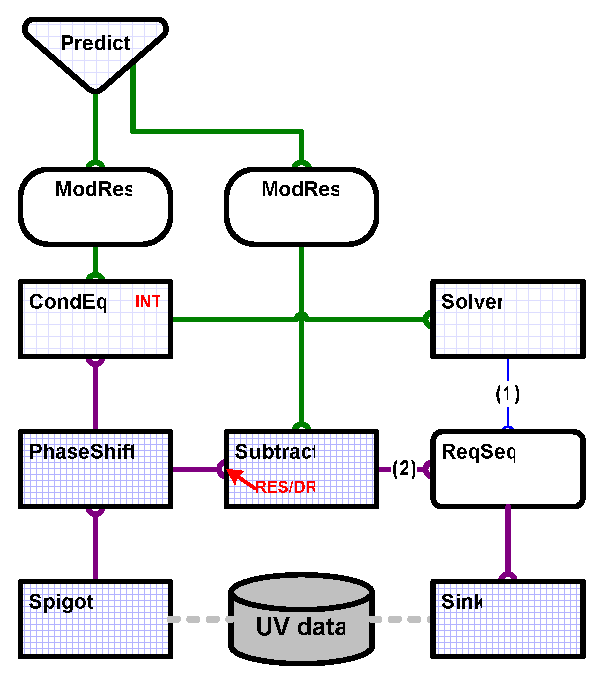
\includegraphics[width=.5\textwidth]{Figures/SolveMultiRes.eps}\\
  %% bb=38 554 327 811
  \end{center}
  \caption{\label{fig:resample}A multiple-resoulution tree employing
  auto-resampling}
  \end{figure}

\subsubsection{Implementation issues}

  For the time being, \qq{Node} only supports integral resamplings. In other
  words, the higher-resolution cells must be perfect tilings of the
  lower-resolution cells. A fail-result is generated otherwise. This keeps
  things simple, and avoids interpolation errors.\footnote{In the future, we
  may add support support arbitrary regridding if needed.} 

  This limitation is less serious than may appear. Resolutions are never chosen
  randomly -- from a tree designer's point of view, they are completely
  deterministic. Current facilities for resolution control (the \qq{ModRes}
  node mentioned below) only allow for integral resolutions. As for the
  original data resolution, it always comes in from the data access nodes
  (\qq{Sink} and \qq{Spigot}), which are tightly coupled: for each snippet of
  data, the \qq{Sink} issues a \Request\ with a \Cells\ corresponding to the
  data layout, while the corresponding \qq{Spigot} is then ready to return a
  \Result\ with the same cells. Thus, the tree designer can always define
  working resolutions for subtrees in terms of integral factors of the original
  data resolution.
  
  Upsampling currently uses linear interpolation. In the future, we may add
  support for more sophisticated resampling.

\subsection{Controlling the resolution}

  The \qq{ModRes} utility node may be used to change resolution mid-tree. A
  \qq{ModRes} always has a single child; upon receiving a \Request\ from its
  parent, it modifies its resolution up or down by a fixed factor (independent
  for each axis), as determined by its node state. The modified \Request\ is
  passed on to its child, and the child's \Result\ is returned directly to the
  parent.

  In the future, we envision an adaptive resolution reducer (ARR) node, which
  adaptively selects a minimum required resolution based on some
  application-specific considerations. These may include:

  \begin{itemize}
  
  \item For solving, the predict tree need only supply enough cells to
  constrain the solution. The minimum resolution can be determined by the
  \qq{Solver} node, and passed along in the \Request\ as a hint to any ARR nodes
  up the tree.
  
  \item For subtracting predicted sources, the cells need only be big enough
  to ensure linearity over a cell. 
  
  \end{itemize}
  
  Note also that the \qq{Identity} node, when configured with a ``Use Request''
  resampling strategy, becomes a {\em resolution coupler}, ensuring resampling
  all results to the requested resolution.

\subsection{How this applies to getResult()}
  \label{sec:getResult}

  Note that the \qq{getResult()} handler discussed above receives two crucial
  pieces of information: a vector of child results, and a \Cells\ (passed by
  ref). The \Cells\ parameter defines the expected result cells, and it is
  set up as follows:

  \begin{itemize}
  
  \item If auto-resampling is not enabled, or the node has no children, then
  this is simply the cells from the \Request. The resolutions of child results,
  if any, are not constrained.
  
  Note that most nodes' contracts specify that ``this node only deals with
  child results at the same resolution'' (this is true, e.g., for all
  \qq{Function} nodes), and leave it up to the tree designer to ensure it (i.e.
  by enabling auto-resampling where necessary). The node's behaviour when a
  contract is violated does not need to be defined (although one can reasonably
  expect an exception to be thrown, leading to a fail-result).

  \item If auto-resampling is enabled, then the resolutions of child results
  are constrained: they will all have the indicated \Cells\ (with the exception
  of resolution-free results, which have no cells). Most nodes are expected to
  return a result at the same resolution.

  \item If auto-resampling is enabled and all child results are
  resolution-free, then the \Cells\ ref is empty. In this case, most nodes'
  result will should be resolution-free as well. In the rare case where the
  node introduces its own time-frequency dependence (e.g. the \qq{UVW} node),
  it should get a \Cells\ from the request.

  \end{itemize}

\section{Function nodes}
\label{sec:Function}

  \qq{Function} is an important subclass of \qq{Node}, representing some
  function of its children's results. The main feature of \qq{Function} is an
  abstract \qq{evaluate()} method, which takes a vector of \Vells\ objects,
  computes some function over them, and returns a \Vells\ result.

  Remember that a \Vells\ is a an $N\times M$ matrix ($\bar{f}=\{f_{ij}\}$) of
  $\RR$ or $\CC$ values, representing a set of sampling or integrations of a
  function $f:\RR^2\rightarrow\RR$ or $f:\RR^2\rightarrow\CC$ over some cells.
  \Vells\ are organized into \VellSet{}s, containing the main value
  $\{f_{ij}\}$, plus an optional set of $K\times S$ $(S=1,2)$ perturbed values
  $\bar{f}_{sk} = \{f^{(sk)}_{ij}\}$, which correspond to $S$ sets of
  perturbations w.r.t. $K$ solvable parameters. A \VellSet\ will also contain
  $S$ vectors of the perturbations themselves, $\{\delta^{(s)}_k\}$.

  The \Result\ of child $l$ will contain $Q_l$ \VellSet{}s. Most of the time,
  $Q_l=1$; when $Q_l>1$, the result represents a multidimensional function
  $f:\RR^2\rightarrow\{\RR\mbox{ or }\CC\}^{Q_l}$. Note that each plane of such
  a function may have its own set of solvable parameters and perturbed values.
  We will use the notation $\bar{f}_{lq}$ to designate the main value for child
  $l$, plane $q$, and $\bar{f}^{(sk)}_{lq}$ to designate the corresponding
  perturbed value for parameter $k$ from set $s$.

  The \qq{evaluate()} method of a \qq{Function}-derived node implements some
  compound function of $L$ child \Vells\ defined over the same \Cells. We will
  designate this function as $F=F(\bar{f}_1,...,\bar{f}_L)$. The value of this
  function is a \Vells\ itself, $\bar{F} = \{F_{ij}\}$, also defined over the
  same \Cells. 

  The \qq{Function} class provides a \qq{getResult()} method that iterates over
  all \Vells\ in its child results, calls \qq{evaluate()} to compute $F$, and
  collect the resulting \Vells\ into an output \Result. The same operation is
  done for all perturbed values. Thus, the \qq{Function} class implements a
  basis for all nodes that calculate a compound function of their children.
  PSS4 includes an automatic code generator (documented elsewhere) that will
  generate a full C++ implementation of a \qq{Function}-derived node class,
  given a symbolic expression for the $F$ function. The kernel also provides a
  toolkit of \qq{Function}s that implement most primitive mathematical
  operations.

\subsection{Dealing with multiple planes}

  Note that an implementation of \qq{evaluate()} defines $F$ for a single set of
  \Vells. When child results contain multiple planes, \qq{Function} deals with
  it as follows:
  
  \begin{itemize}
  
  \item If all child results contain the same number of planes $Q$
  $(Q=Q_1=...=Q_L)$, the function $F$ is applied separately to each plane 
  $q=1...Q$.

  \item Child results with a different number of planes are supported in only
  one scenario: some results may have 1 plane, and some may have $Q>1$ planes,
  but $Q$ must be the same for all multi-planar results (a fail is generated if
  this condition is not met). Results with 1 plane are then artificially
  expanded to $Q$ planes by reusing the same \VellSet\ for all planes from 1 to
  $Q$. (This is roughly similar to scalar-vector operations in Glish.)

  \end{itemize}
  
\subsection{Dealing with perturbed values}

  Each plane (aka \VellSet) $q$ of result $l$ may contain a number of perturbed
  values. These are also evaluated. Note that the set of parameters (identified
  by spids) with respect to which the values are perturbed is not necessarily
  the same for each child result or plane, in fact, some planes or results may
  contain no perturbed values at all.
  
  To simplify the description here, let's remember that \qq{Function} deals
  with multiple result planes independently, on a plane-by-plane basis (see
  above). Hence, we'll assume we're dealing with only one plane, and $l$ child
  results for that plane. We'll also forget about multiple perturbation sets,
  since those are all dealt with in the same way. 

  \qq{Function} starts by figuring out all the spids present in the \VellSet{}s
  of the children. Thus, it ends up with a list of spids,
  $(\kappa_1,...,\kappa_n)$, which is simply the union of the spid sets from
  each child's \VellSet. For each spid $\kappa_i$, it then needs to compute the
  perturbed value of $F$ with respect to parameter $\kappa_i$
  $(\bar{F}^{(\kappa_i)})$, based on the perturbed \Vells\
  $(\bar{f}^{(k)})$ found in the child \VellSet{}s.

  This is done by calling \qq{evaluate()} $n$ times to compute
  $\bar{F}^{(\kappa_i)}$ for each $\kappa_i$, while selecting the input \Vells\
  from each child's result as follows. If spid $\kappa_i$ is present in the
  list of spids for  the \VellSet\ of child $l$, the perturbed value
  $\bar{f}^{(lk)}$ is used (where $k$ corresponds to spid $\kappa_i$).
  Otherwise, the main value $\bar{f}_l$ is used.

  If this seems complicated at first glance, remember that the end result is
  quite simple. A \qq{Function} node computes some function over its children's
  results. If the subtrees above the node contain solvable parameters, then
  perturbed values of that same function {\bf w.r.t. all the solvable
  parameters} must be computed as well, based on perturbed values returned by
  the children. Everything else follows from this simple requirement.

\subsection{Restrictions on child results}
   
  A \qq{Function} node imposes certain restrictions on the structure of its child
  results, which the tree designer should be aware of. If the results do not
  have the right layout, a fail is always generated.
  
  \begin{itemize}
  
  \item The first restriction has already been covered above -- all results must have
  the same number of planes, or must be a mix of $Q$ planes and single planes.
  \qq{Composer} and \qq{Selector} nodes should be placed appropriately to ensure
  this.
  
  \item The second restriction has also been mentioned -- all results must have
  the same \Cells. Auto-resampling may need to be enabled to ensure this. This
  implies that all \Vells\ in the results will have either the same $M\times N$
  shape, or will be scalars (i.e. no time-frequency dependence).
  
  \item The child results must be either all samplings or all integrations. The
  two types cannot be mixed in the same expression.

  \item The next restriction involves the values of the perturbations
  $(\delta_\kappa)$ themselves. When $F$ is evaluated over perturbed values for
  parameter $\kappa$, and these perturbed values appear in more than one
  \VellSet, the result is sensible only when the perturbation
  $\delta_\kappa$ is the same thoroughout. 

  \item Finally, if more than one perturbed value set is used (think
  double-differencing), \qq{Function} requires that all child results have the
  same number of sets, though any child may always return zero sets (no
  perturbed values at all).

  \end{itemize}
  
  Note that the last two restrictions are almost always met automatically,
  since the perturbations $\delta_\kappa$ are usually determined by the
  parameters (i.e. \qq{Parm} nodes) themselves. Single- or double-differencing
  is determined by the value of \qq{calc\_deriv} in the \Request, which is also
  the same for all children. You'd be hard-pressed to construct a tree that
  didn't meet these two restrictions. Nevertheless, it's something to keep in
  mind in case you see \qq{Function} nodes failing unexpectedly.

\subsection{Implementing evaluate(): Vells arithmetic}
  \label{sec:vells}

  The \qq{evaluate()} method is defined as follows:
  
  \begin{verbatim}  
  virtual Vells evaluate (const Request &req,
                          const LoShape &shape,
                          const std::vector<const Vells*> &args);
  \end{verbatim}
  
  The \qq{req} argument is simply the original \Request. \qq{shape} indicates
  the shape of the output \Vells\ (i.e. the shape of the result \Cells, see
  \ref{sec:getResult}). The last parameter is a vector of pointers to argument
  \Vells, which \qq{Function} sets up for each call so that the correct
  combination of main values and perturbed values is used. Note that the
  resulting \Vells\ is returned by value; this is a very fast operation, since
  \Vells\ utilizes copy-on-write for its contents.

  \begin{table}[th]
  \begin{center}\begin{tabular}{|p{.25\textwidth}p{.7\textwidth}|}
  
  \tablesubheading{2}{basic arithmetic:}\\
  \qq{-} & unary negation\\
  \qq{+ - * /} & standard binary arithmetic operators\\
  
  \tablesubheading{2}{in-place arithmetic:}\\
  \qq{+= -= *= /=} & arithmetic, modifies the left-hand \Vells\ in-place\\
  
  \tablesubheading{2}{unary functions, $\RR\rightarrow\RR$ and
                      $\CC\rightarrow\CC$:}\\
  \qq{exp() log() log10()} & $e^x$, $\ln{x}$, $\log{x}$\\
  \qq{sqr() sqrt()} & $x^2$, $\sqrt{x}$ \\
  \qq{pow2()}...\qq{pow8()} & $x^2...x^8$\\
  \qq{sin() cos() tan()} & sine, cosine, tangent \\
  \qq{sinh() cosh() tanh()} & hyperbolic sine, cosine, tangent \\
  \qq{conj()} & complex conjugate \\
  
  \tablesubheading{2}{unary functions, $\RR\rightarrow\RR$ only:}\\
  \qq{ceil()} & nearest integer $\ge x$\\
  \qq{floor()} & nearest integer $\le x$\\
  \qq{acos() asin() atan()} & arccosine, arcsine, arctangent \\
  
  \tablesubheading{2}{unary functions, $\RR\rightarrow\RR$ or 
                      $\CC\rightarrow\RR$:}\\
  \qq{abs() fabs()} & absolute value $|x|$ (both names are equivalent)\\
  \qq{norm()} & norm: $|x|^2$\\
  \qq{arg()} & argument of a complex number (the $\phi$ in $x=|x|e^{i\phi}$)\\
  \qq{real() imag()} & real and imaginary parts\\

  \tablesubheading{2}{array reductions:}\\ 
  
  \qq{min() max() mean() sum() product()} & these reduce the argument
  (presumbaly, an array \Vells) to a single scalar. Note that \qq{min()} and
  \qq{max()} are only defined for real arguments.\\

  \tablesubheading{2}{binary functions:}\\
  \qq{tocomplex()} & $x+iy$\\
  \qq{pow()} & $x^y$ \\
  \qq{atan2()} & $\arctan(y/x)$, also defined for $x=0$\\
  \qq{posdiff()} & angular difference: for two angles $x,y$ in the range
  $[-\pi,\pi]$, returns $x-y$ renormalized into $[-\pi,\pi]$ by adding $\pm2\pi$ as
  necessary.\\
  
  \hline
  \end{tabular}\end{center}
  
  {\em Note: some \Vells\ functions are defined for real arguments only.
  Applying them to a complex \Vells\ will result in a fail.}

  \caption{\label{table:vellsmath}Available \qq{Vells} operations}
  \end{table}

  Implementations can take advantage of {\em \Vells\ math}. \Vells\ is an
  intelligent wrapper for real or complex 2D arrays or scalars, with overloaded
  operators and functions for basic math and implicit conversion from scalar
  values to a \Vells. It provides automatic type promotion, and can also
  implictly ``expand'' a scalar to an array. For example, the doubled product
  of two \Vells\ \qq{a} and \qq{b} may be obtained simply by stating
  \qq{c=2*a*b}. This notation conveniently hides a lot of messy processing:
  real \Vells\ are automatically promoted to complex if the other argument is
  complex, scalars are expanded to arrays if the other argument is an array,
  and the operation is performed on an element-by-element basis.\footnote{An
  exception is thrown if two array \Vells\ have a different  shape. Note that
  having the same \Cells\ in all child results ensures the same shape for all
  \Vells.}  As another example, here's an actual implementation of
  \qq{evaluate()} for the \qq{Cos} node (computes cosine of child result):

  \begin{verbatim}
  Vells Cos::evaluate (const Request&,const LoShape &,
                       const vector<const Vells*>& args)
  {
    return cos(*(args[0]));
  }
  \end{verbatim}
  
  Table~\ref{table:vellsmath} lists all the primitive operators and functions 
  available with the \qq{Vells} class. Most of these operate on \qq{const}
  arguments and return a new \Vells\ object by value. The exception are 
  in-place operators (\qq{"+="} and friends), which modify a \qq{Vells} in
  place and return it as \qq{"Vells\&"} (these obviously require a
  non-\qq{const} argument). The C++ syntax allows one to freely combine
  primitive operations into complicated expressions, while the compiler takes
  care of creating and destroying intermediate \Vells\ objects as appropriate.

  \subsubsection{Copy-on-write specifics}

  Since \Vells\ employ copy-on-write, using \Vells\ math for complicated
  expressions incurs very little overhead in comparison to an ``optimized''
  implementation with explicit looping over array elements. The amount of
  messy coding saved, on the other hand, is huge. 
  
  Copy-on-write means that when one \Vells\ is assigned to or initialized from
  another \Vells, the two start off sharing the same data. This makes 
  copy/assignment operations very economical, since the underlying data array 
  is not copied. Any subsequent attempts to modify either \Vells\ will cause a
  true private copy of the data to be made. Thus, copying of data arrays is
  deferred until it is actually needed (which may be never). 

  Consider, for example, an implementation of \qq{Add:evaluate()}. The \qq{Add}
  node adds the results of any number of children:

  \begin{verbatim}  
  Vells Add::evaluate (const Request&, const LoShape&,
                       const vector<const Vells*>& args)
  {
    if( args.empty() )
      return Vells(0.);
    Vells result(*args[0],DMI::READONLY);
    for( uint i=1; i<args.size(); i++ )
      result += *(args[i]);
    return result;
  }
  \end{verbatim}  
  
  The \qq{result} \Vells\ is initialized from the first argument \Vells, and
  shares data with it. As soon as the second argument is added in, a private 
  copy of \qq{result}'s data is implicitly created. If, however, only one
  argument is passed in to begin with, the \qq{result} will still share data
  with it when returned.

%  The \MeqServer\ object provides an interface to the MeqTree kernel. It 
  
  


\chapter{The MeqServer Interface}
\label{chap:meqserver}
\label{sec:meqserver}
\label{sec:meqforest}


%  The \MeqServer\ object provides an interface to the MeqTree kernel. It 
  
  
  \begin{figure}[th]
  \begin{center}
  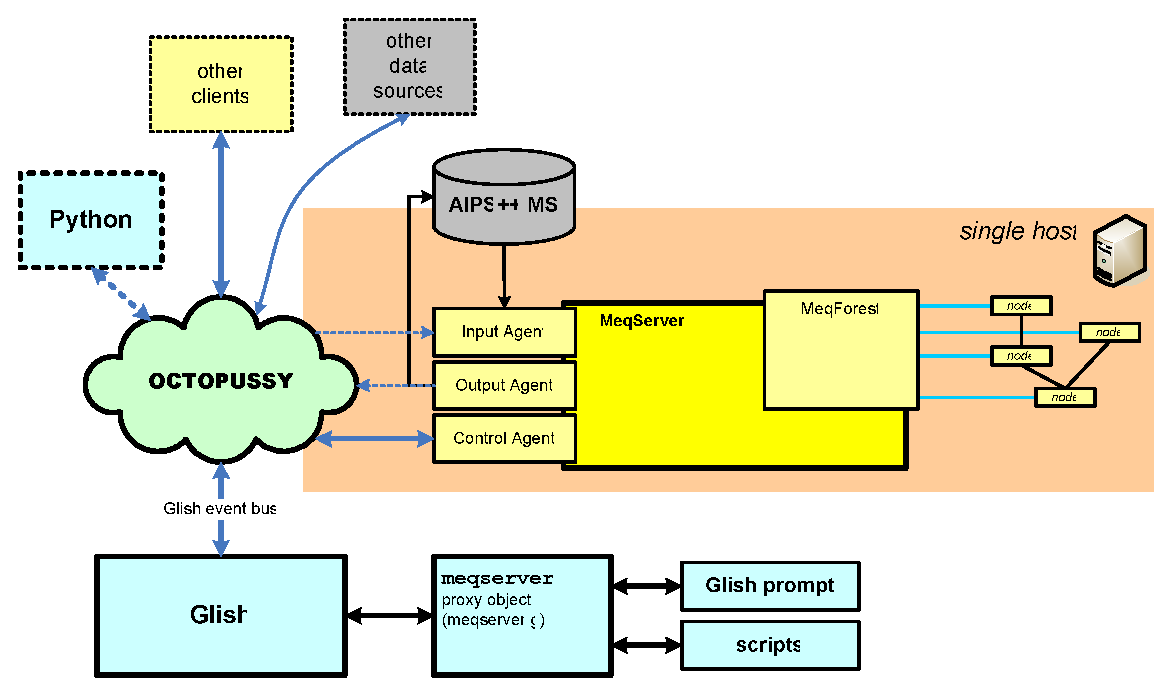
\includegraphics[width=.92\textwidth]{Figures/MeqServer.eps}\\
  %% bb=38 554 327 811
  \end{center}
  \caption{\label{fig:meqserver}MeqServer and MeqTree control}
  \end{figure}


\end{document}
